% Preamble
\documentclass[11pt]{article}

% Packages
\usepackage{amsmath}
\usepackage{amssymb}
\usepackage{tikz}
\usetikzlibrary{arrows,arrows.meta,positioning,calc,petri}
\usepackage{adjustbox}
\usepackage{enumitem}
\usepackage{listings}
\usepackage[ruled,vlined]{algorithm2e}
\SetKwRepeat{Do}{do}{until}%
\newtheorem{theorem}{Theorem}

% Document
\begin{document}
    % P/T reductions
    \section*{Rule A: Sequential transition removal}\label{sec:rule_a}
Rule~A merges sequential transitions, i.e.\ a transition and another transition that must precede or follow it.
Rule~A is equivalent to a pre (or post) agglomeration with exactly one producer (or consumer) with a weight of 1.
The two variants of Rule~A can be seen in Figure~\ref{fig:rule_a_pre} and Figure~\ref{fig:rule_a_post}.

\begin{theorem}\label{theorem:rule_a}
    The two variants of Rule~A in Figure~\ref{fig:rule_a_pre} and Figure~\ref{fig:rule_a_post} are both correct for LTL\textbackslash X cardinality properties.
\end{theorem}

\begin{figure}[h]
    \centering
    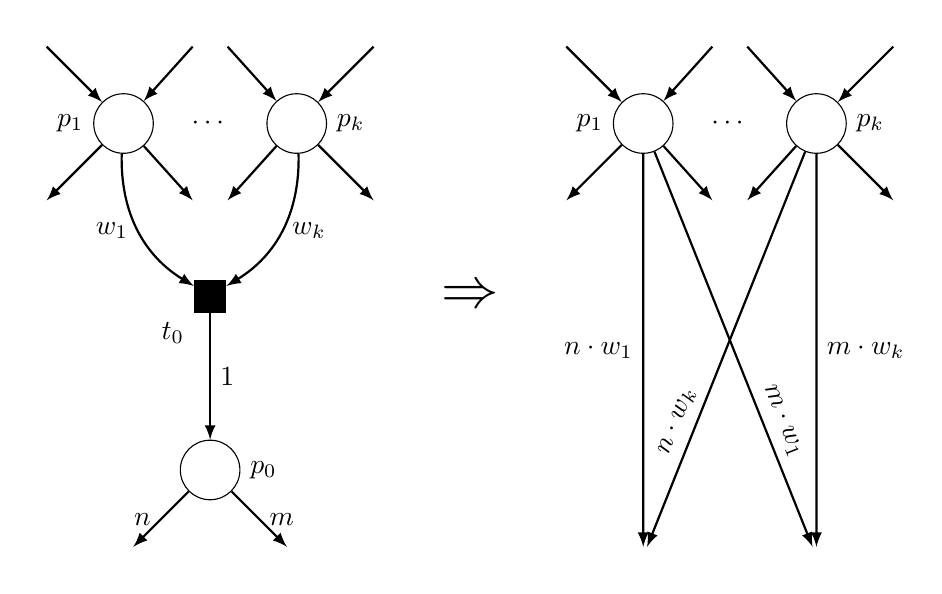
\begin{tikzpicture}[scale=1.1]
        %%%% Before =====================================
        \begin{scope}
            % Places
            \node[place,label=right:$p_0$] (p0) at (0, -2) {};
            \node[place,label=left:$p_1$] (p1) at (-1, 2) {};
            \node[place,label=right:$p_k$] (pk) at (1, 2) {};
            \node at (0, 2) {$\cdots$};

            % Transitions
            \node[transition,fill=black,label=below left:$t_0$] (t0) at (0, 0) {};

            % Invisible transitions
            \node (p1pre1) at (-2, 3) {};
            \node (p1pre2) at (-.1, 3) {};
            \node (pkpre1) at (.1, 3) {};
            \node (pkpre2) at (2, 3) {};
            \node (p1post1) at (-2, 1) {};
            \node (p1post2) at (-.1, 1) {};
            \node (pkpost1) at (.1, 1) {};
            \node (pkpost2) at (2, 1) {};
            \node (p0post1) at (-1, -3) {};
            \node (p0post2) at (1, -3) {};

            % Arcs
            \draw[-latex,thick] (p1pre1) -- (p1);
            \draw[-latex,thick] (p1pre2) -- (p1);
            \draw[-latex,thick] (pkpre1) -- (pk);
            \draw[-latex,thick] (pkpre2) -- (pk);
            \draw[-latex,thick] (p1) -- (p1post1);
            \draw[-latex,thick] (p1) -- (p1post2);
            \draw[-latex,thick] (pk) -- (pkpost1);
            \draw[-latex,thick] (pk) -- (pkpost2);
            \draw[-latex,thick] (p1) edge[bend right] node[left] {$w_1$} (t0);
            \draw[-latex,thick] (pk) edge[bend left] node[right] {$w_k$} (t0);
            \draw[-latex,thick] (p0) -- node[left] {$n$} (p0post1);
            \draw[-latex,thick] (p0) -- node[right] {$m$} (p0post2);
            \draw[-latex,thick] (t0) -- node[right] {$1$} (p0);

        \end{scope}

        %%%% Arrow and conditions =======================
        \node (arrow) at (3,0) {\huge$\Rightarrow$};

        %%%% After ======================================
        \begin{scope}[shift={(6,0)}]
            % Places
            \node[place,label=left:$p_1$] (p1) at (-1, 2) {};
            \node[place,label=right:$p_k$] (pk) at (1, 2) {};
            \node at (0, 2) {$\cdots$};

            % Invisible transitions
            \node (p1pre1) at (-2, 3) {};
            \node (p1pre2) at (-.1, 3) {};
            \node (pkpre1) at (.1, 3) {};
            \node (pkpre2) at (2, 3) {};
            \node (p1post1) at (-2, 1) {};
            \node (p1post2) at (-.1, 1) {};
            \node (pkpost1) at (.1, 1) {};
            \node (pkpost2) at (2, 1) {};
            \node (p0post1) at (-1, -3) {};
            \node (p0post2) at (1, -3) {};

            % Arcs
            \draw[-latex,thick] (p1pre1) -- (p1);
            \draw[-latex,thick] (p1pre2) -- (p1);
            \draw[-latex,thick] (pkpre1) -- (pk);
            \draw[-latex,thick] (pkpre2) -- (pk);
            \draw[-latex,thick] (p1) -- (p1post1);
            \draw[-latex,thick] (p1) -- (p1post2);
            \draw[-latex,thick] (pk) -- (pkpost1);
            \draw[-latex,thick] (pk) -- (pkpost2);
            \draw[-latex,thick] (p1) -- node[left] {$n\cdot w_1$} (p0post1);
            \draw[-latex,thick] (p1) edge[sloped, above, pos=0.7] node {$m\cdot w_1$} (p0post2);
            \draw[-latex,thick] (pk) edge[sloped, above, pos=0.7] node {$n\cdot w_k$} (p0post1);
            \draw[-latex,thick] (pk) -- node[right] {$m\cdot w_k$} (p0post2);
        \end{scope}
    \end{tikzpicture}
    \vspace{1cm}

    \begin{adjustbox}{center}
        \begin{tabular}{|p{70mm}|p{62mm}|} \hline
        Precondition & Update \\ \hline
        Fix $p_0$ and $t_0$ where ${}^\bullet t_0=\{p_1,\dotsc,p_k\}$ s.t.:
        \begin{itemize}[leftmargin=10mm]
            \item[A1)] $t_0^\bullet=\{p_0\}$ and $\boxplus(t_0, p_0)=1$
            \item[A2)] ${}^\bullet p_0=\{t_0\}$ and $p_0\notin\{p_1,\dotsc,p_k\}$
            \item[A3)] $p_0^\circ=p_1^\circ=\dots=p_k^\circ={}^\circ t_0=\emptyset$
            \item[A4)] $\{p_0, p_1,\dotsc,p_k\}\cap places(\varphi)=\emptyset$
            \item[A5)] $M_0(p_0)=0$
        \end{itemize} &
        \begin{itemize}[leftmargin=10mm]
            \item[UA1)] For all $t\in p_0^\bullet$ and all $p\in\{p_1,\dotsc,p_k\}$ set $\boxminus'(p,t):=\boxminus(p,t)+\boxminus(p_0,t)\cdot\boxminus(p,t_0)$
            \item[UA2)] Remove $p_0$ and $t_0$
        \end{itemize} \\ \hline
        \end{tabular}
    \end{adjustbox}
    \caption{Rule A: Sequential transition removal (pre)}
    \label{fig:rule_a_pre}
\end{figure}

\begin{figure}[h]
    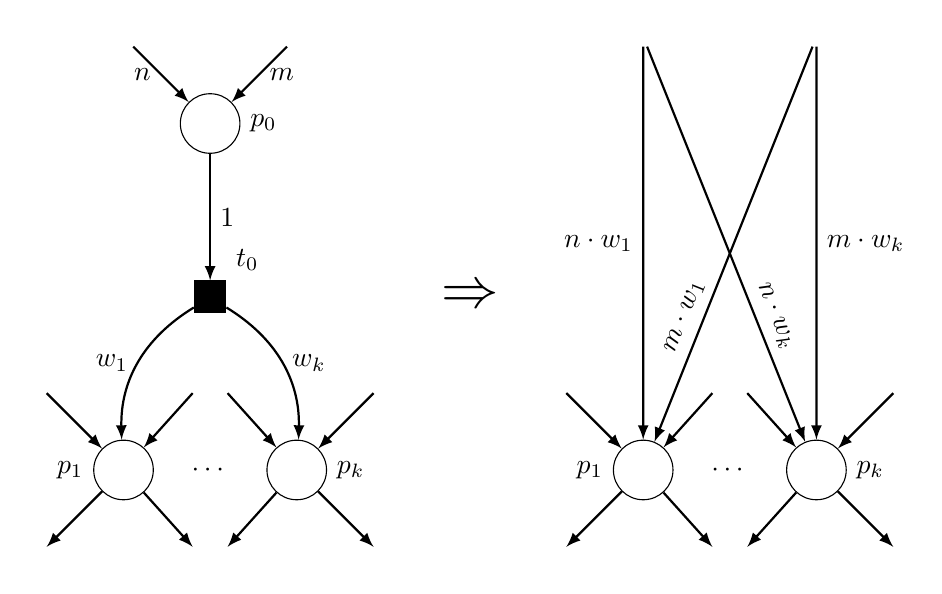
\begin{tikzpicture}[scale=1.1]
        %%%% Before =====================================
        \begin{scope}
            % Places
            \node[place,label=right:$p_0$] (p0) at (0, 2) {};
            \node[place,label=left:$p_1$] (p1) at (-1, -2) {};
            \node[place,label=right:$p_k$] (pk) at (1, -2) {};
            \node at (0, -2) {$\cdots$};

            % Transitions
            \node[transition,fill=black,label=above right:$t_0$] (t0) at (0, 0) {};

            % Invisible transitions
            \node (p0pre1) at (-1, 3) {};
            \node (p0pre2) at (1, 3) {};
            \node (p1pre1) at (-2, -1) {};
            \node (p1pre2) at (-.1, -1) {};
            \node (pkpre1) at (.1, -1) {};
            \node (pkpre2) at (2, -1) {};
            \node (p1post1) at (-2, -3) {};
            \node (p1post2) at (-.1, -3) {};
            \node (pkpost1) at (.1, -3) {};
            \node (pkpost2) at (2, -3) {};

            % Arcs
            \draw[-latex,thick] (p0pre1) -- node[left] {$n$} (p0);
            \draw[-latex,thick] (p0pre2) -- node[right] {$m$} (p0);
            \draw[-latex,thick] (p0) -- node[right] {$1$} (t0);
            \draw[-latex,thick] (t0) edge[bend right] node[left] {$w_1$} (p1);
            \draw[-latex,thick] (t0) edge[bend left] node[right] {$w_k$} (pk);
            \draw[-latex,thick] (p1pre1) -- (p1);
            \draw[-latex,thick] (p1pre2) -- (p1);
            \draw[-latex,thick] (pkpre1) -- (pk);
            \draw[-latex,thick] (pkpre2) -- (pk);
            \draw[-latex,thick] (p1) -- (p1post1);
            \draw[-latex,thick] (p1) -- (p1post2);
            \draw[-latex,thick] (pk) -- (pkpost1);
            \draw[-latex,thick] (pk) -- (pkpost2);

        \end{scope}

        %%%% Arrow and conditions =======================
        \node (arrow) at (3,0) {\huge$\Rightarrow$};

        %%%% After ======================================
        \begin{scope}[shift={(6,0)}]
            % Places
            \node[place,label=left:$p_1$] (p1) at (-1, -2) {};
            \node[place,label=right:$p_k$] (pk) at (1, -2) {};
            \node at (0, -2) {$\cdots$};

            % Invisible transitions
            \node (p0pre1) at (-1, 3) {};
            \node (p0pre2) at (1, 3) {};
            \node (p1pre1) at (-2, -1) {};
            \node (p1pre2) at (-.1, -1) {};
            \node (pkpre1) at (.1, -1) {};
            \node (pkpre2) at (2, -1) {};
            \node (p1post1) at (-2, -3) {};
            \node (p1post2) at (-.1, -3) {};
            \node (pkpost1) at (.1, -3) {};
            \node (pkpost2) at (2, -3) {};

            % Arcs
            \draw[-latex,thick] (p0pre1) -- node[left] {$n\cdot w_1$} (p1);
            \draw[-latex,thick] (p0pre1) edge[sloped, above, pos=0.7] node {$n\cdot w_k$} (pk);
            \draw[-latex,thick] (p0pre2) edge[sloped, above, pos=0.7] node {$m\cdot w_1$} (p1);
            \draw[-latex,thick] (p0pre2) -- node[right] {$m\cdot w_k$} (pk);
            \draw[-latex,thick] (p1pre1) -- (p1);
            \draw[-latex,thick] (p1pre2) -- (p1);
            \draw[-latex,thick] (pkpre1) -- (pk);
            \draw[-latex,thick] (pkpre2) -- (pk);
            \draw[-latex,thick] (p1) -- (p1post1);
            \draw[-latex,thick] (p1) -- (p1post2);
            \draw[-latex,thick] (pk) -- (pkpost1);
            \draw[-latex,thick] (pk) -- (pkpost2);
        \end{scope}
    \end{tikzpicture}
    \vspace{1cm}

    \begin{adjustbox}{center}
        \begin{tabular}{|p{70mm}|p{62mm}|} \hline
        Precondition & Update \\ \hline
        Fix $p_0$ and $t_0$ where $t_0^\bullet=\{p_1,\dotsc,p_k\}$ s.t.:
        \begin{itemize}[leftmargin=10mm]
            \item[A1)] ${}^\bullet t_0=\{p_0\}$ and $\boxminus(p_0, t_0)=1$
            \item[A2)] $p_0^\bullet=\{t_0\}$ and $p_0\notin\{p_1,\dotsc,p_k\}$
            \item[A3)] $p_0^\circ=p_1^\circ=\dots=p_k^\circ={}^\circ t_0=\emptyset$
            \item[A4)] $\{p_0, p_1,\dotsc,p_k\}\cap places(\varphi)=\emptyset$
        \end{itemize} &
        \begin{itemize}[leftmargin=10mm]
            \item[UA1)] For all $p\in\{p_1,\dotsc,p_k\}$ change the initial marking s.t.\ $M_0'(p):=M_0(p)+M_0(p_0)\cdot\boxplus(t_0, p)$
            \item[UA2)] For all $t\in{}^\bullet p_0$ and all $p\in\{p_1,\dotsc,p_k\}$ set $\boxplus'(t,p):=\boxplus(t,p)+\boxplus(t,p_0)\cdot\boxplus(t_0,p)$
            \item[UA3)] Remove $p_0$ and $t_0$
        \end{itemize} \\ \hline
        \end{tabular}
    \end{adjustbox}
    \caption{Rule A: Sequential transition removal (post)}
    \label{fig:rule_a_post}
\end{figure}

    \clearpage
    \section*{Rule B: Sequential place removal}\label{sec:rule_b}
Rule~B merges two transitions surrounding a place with no other transitions than the two.
Rule~B is equivalent to an agglomeration with exactly one producer and one consumer, but allow them to have different weights.
Hence, there is a pre- and post-agglomeration variant of Rule~B defined in Figure~\ref{fig:rule_b_pre} and Figure~\ref{fig:rule_b_post}, respectively.

\begin{theorem}\label{theorem:rule_b}
    The two variants of Rule~B in Figure~\ref{fig:rule_b_pre} and Figure~\ref{fig:rule_b_post} are both correct for LTL\textbackslash X.
\end{theorem}

\begin{figure}[h]
    \centering
    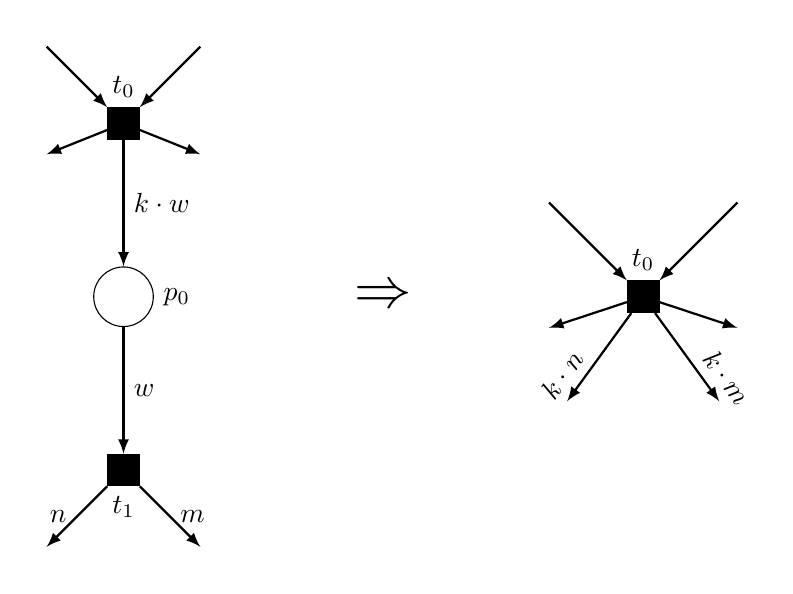
\begin{tikzpicture}[scale=1.1]
        %%%% Before =====================================
        \begin{scope}
            % Places
            \node[place,label=right:$p_0$] (p0) at (0, 0) {};

            % Transitions
            \node[transition,fill=black,label=above:$t_0$] (t0) at (0, 2) {};
            \node[transition,fill=black,label=below:$t_1$] (t1) at (0, -2) {};

            % Invisible places
            \node (t0pre1) at (-1, 3) {};
            \node (t0pre2) at (1, 3) {};
            \node (t0post1) at (-1, 1.6) {};
            \node (t0post2) at (1, 1.6) {};
            \node (t1post1) at (-1, -3) {};
            \node (t1post2) at (1, -3) {};

            % Arcs
            \draw[-latex,thick] (t0pre1) -- (t0);
            \draw[-latex,thick] (t0pre2) -- (t0);
            \draw[-latex,thick] (t0) -- (t0post1);
            \draw[-latex,thick] (t0) -- (t0post2);
            \draw[-latex,thick] (t0) -- node[right] {$k\cdot w$} (p0);
            \draw[-latex,thick] (p0) -- node[right] {$w$} (t1);
            \draw[-latex,thick] (t1) -- node[left] {$n$} (t1post1);
            \draw[-latex,thick] (t1) -- node[right] {$m$} (t1post2);
        \end{scope}

        %%%% Arrow and conditions =======================
        \node (arrow) at (3,0) {\huge$\Rightarrow$};

        %%%% After ======================================
        \begin{scope}[shift={(6,0)},scale=1.2]
            % Transitions
            \node[transition,fill=black,label=above:$t_0$] (t0) at (0, 0) {};

            % Invisible places
            \node (t0pre1) at (-1, 1) {};
            \node (t0pre2) at (1, 1) {};
            \node (t0post1) at (-1, -.33) {};
            \node (t0post2) at (1, -.33) {};
            \node (t1post1) at (-.8, -1.1) {};
            \node (t1post2) at (.8, -1.1) {};

            % Arcs
            \draw[-latex,thick] (t0pre1) -- (t0);
            \draw[-latex,thick] (t0pre2) -- (t0);
            \draw[-latex,thick] (t0) -- (t0post1);
            \draw[-latex,thick] (t0) -- (t0post2);
            \draw[-latex,thick] (t0) edge[sloped] node[above left] {$k\cdot n$} (t1post1);
            \draw[-latex,thick] (t0) edge[sloped] node[above right] {$k\cdot m$} (t1post2);
        \end{scope}
    \end{tikzpicture}
    \vspace{1cm}

    \begin{adjustbox}{center}
        \begin{tabular}{|p{70mm}|p{62mm}|} \hline
        Precondition & Update \\ \hline
        Fix $p_0$ and $t_0,t_1$ where $t_0\neq t_1$ s.t.:
        \begin{itemize}[leftmargin=10mm]
            \item[B1)] ${}^\bullet p_0=\{t_0\}, p_0^\bullet=\{t_1\},{}^\bullet t_1=\{p_0\}$
            \item[B2)] $\boxplus(t_0,p_0)=k\cdot\boxminus(p_0, t_1)$ for $k\geq 1$
            \item[B3)] $p_0^\circ ={}^\circ t_0={}^\circ t_1=\emptyset$
            \item[B4)] $p_0\notin places(\varphi)$
            \item[B5)] $p^\circ =\emptyset$ and $p\notin places(\varphi)$ for all $p\in t_1^\bullet$
        \end{itemize} &
        \begin{itemize}[leftmargin=10mm]
            \item[UB1)] For all $p\in P\setminus\{p_0\}$ set $M_0'(p):=M_0(p)+\lfloor M_0(p_0)/\boxminus(p_0,t_1)\rfloor\cdot\boxplus(t_1,p)$
            \item[UB2)] For all $p\in P\setminus\{p_0\}$ set $\boxplus'(t_0,p):=\boxplus(t_0,p)+k\cdot\boxplus(t_1,p)$
            \item[UB3)] Remove $p_0$ and $t_1$
        \end{itemize} \\ \hline
        \end{tabular}
    \end{adjustbox}
    \caption{Rule B: Sequential place removal (pre)}
    \label{fig:rule_b_pre}
\end{figure}

\begin{figure}[h]
    \centering
    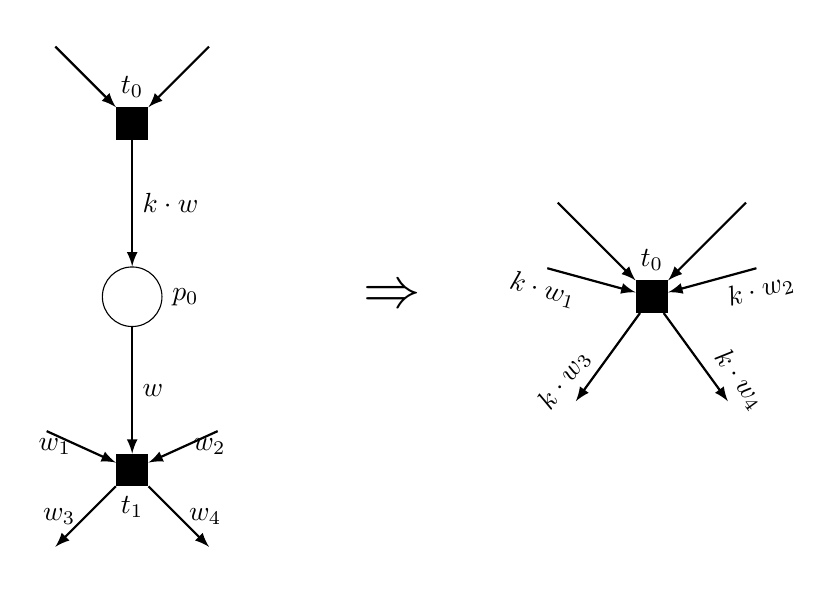
\begin{tikzpicture}[scale=1.1]
        %%%% Before =====================================
        \begin{scope}
            % Places
            \node[place,label=right:$p_0$] (p0) at (0, 0) {};

            % Transitions
            \node[transition,fill=black,label=above:$t_0$] (t0) at (0, 2) {};
            \node[transition,fill=black,label=below:$t_1$] (t1) at (0, -2) {};

            % Invisible places
            \node (t0pre1) at (-1, 3) {};
            \node (t0pre2) at (1, 3) {};
            \node (t1pre1) at (-1.1, -1.5) {};
            \node (t1pre2) at (1.1, -1.5) {};
            \node (t1post1) at (-1, -3) {};
            \node (t1post2) at (1, -3) {};

            % Arcs
            \draw[-latex,thick] (t0pre1) -- (t0);
            \draw[-latex,thick] (t0pre2) -- (t0);
            \draw[-latex,thick] (t0) -- node[right] {$k\cdot w$} (p0);
            \draw[-latex,thick] (p0) -- node[right] {$w$} (t1);
            \draw[-latex,thick] (t1pre1) -- node[left] {$w_1$} (t1);
            \draw[-latex,thick] (t1pre2) -- node[right] {$w_2$} (t1);
            \draw[-latex,thick] (t1) -- node[left] {$w_3$} (t1post1);
            \draw[-latex,thick] (t1) -- node[right] {$w_4$} (t1post2);
        \end{scope}

        %%%% Arrow and conditions =======================
        \node (arrow) at (3,0) {\huge$\Rightarrow$};

        %%%% After ======================================
        \begin{scope}[shift={(6,0)},scale=1.2]
        % Transitions
        \node[transition,fill=black,label=above:$t_0$] (t0) at (0, 0) {};

        % Invisible places
        \node (t0pre1) at (-1, 1) {};
        \node (t0pre2) at (1, 1) {};
        \node (t1pre1) at (-1.1, .3) {};
        \node (t1pre2) at (1.1, .3) {};
        \node (t1post1) at (-.8, -1.1) {};
        \node (t1post2) at (.8, -1.1) {};

        % Arcs
        \draw[-latex,thick] (t0pre1) -- (t0);
        \draw[-latex,thick] (t0pre2) -- (t0);
        \draw[-latex,thick] (t1pre1) edge[sloped] node[below left] {$k\cdot w_1$} (t0);
        \draw[-latex,thick] (t1pre2) edge[sloped] node[below right] {$k\cdot w_2$} (t0);
        \draw[-latex,thick] (t0) edge[sloped] node[above left] {$k\cdot w_3$} (t1post1);
        \draw[-latex,thick] (t0) edge[sloped] node[above right] {$k\cdot w_4$} (t1post2);
        \end{scope}
    \end{tikzpicture}
    \vspace{1cm}

    \begin{adjustbox}{center}
        \begin{tabular}{|p{70mm}|p{62mm}|} \hline
        Precondition & Update \\ \hline
        Fix $p_0$ and $t_0,t_1$ where $t_0\neq t_1$ s.t.:
        \begin{itemize}[leftmargin=10mm]
            \item[B1)] ${}^\bullet p_0=\{t_0\}, p_0^\bullet=\{t_1\},t_0^\bullet=\{p_0\}$
            \item[B2)] $\boxplus(t_0,p_0)=k\cdot\boxminus(p_0, t_1)$ for $k\geq 1$
            \item[B3)] $p_0^\circ ={}^\circ t_0={}^\circ t_1=\emptyset$
            \item[B4)] $p_0\notin places(\varphi)$ and $M_0(p_0)=0$
            \item[B5)] $p^\circ =\emptyset$ and $p\notin places(\varphi)$ for all $p\in{}^\bullet t_0$
        \end{itemize} &
        \begin{itemize}[leftmargin=10mm]
            \item[UB1)] For all $p\in P\setminus\{p_0\}$ set $\boxminus'(p,t_0):=\boxminus(p,t_0)+k\cdot\boxminus(p,t_1)$
            \item[UB2)] For all $p\in P\setminus\{p_0\}$ set $\boxplus'(t_0,p):=\boxplus(t_0,p)+k\cdot\boxplus(t_1,p)$
            \item[UB3)] Remove $p_0$ and $t_1$
        \end{itemize} \\ \hline
        \end{tabular}
    \end{adjustbox}
    \caption{Rule B: Sequential place removal (post)}
    \label{fig:rule_b_post}
\end{figure}
    \clearpage
    \section*{Rule C: Parallel Places}\label{sec:rule_c}
When two places are parallel to each other and one may accumulate tokens, Rule~C will remove it.
See Figure~\ref{fig:rule_c}.
By convention $\min\emptyset=-\infty$ and $\max\emptyset=\infty$.
The fraction $d$ describes how fast tokens can be consumed from $p_2$ compared to $p_1$,
while $f$ describes how slow tokens can be fed to $p_2$ compared to $p_1$.
If $d\leq f$ then $p_2$ is always fed faster than it is emptied compared to $p_1$,
which means $p_2$ can be removed, since it will always be $p_1$ which is missing tokens and disables their consumers.

\begin{figure}[h!]
    \centering
    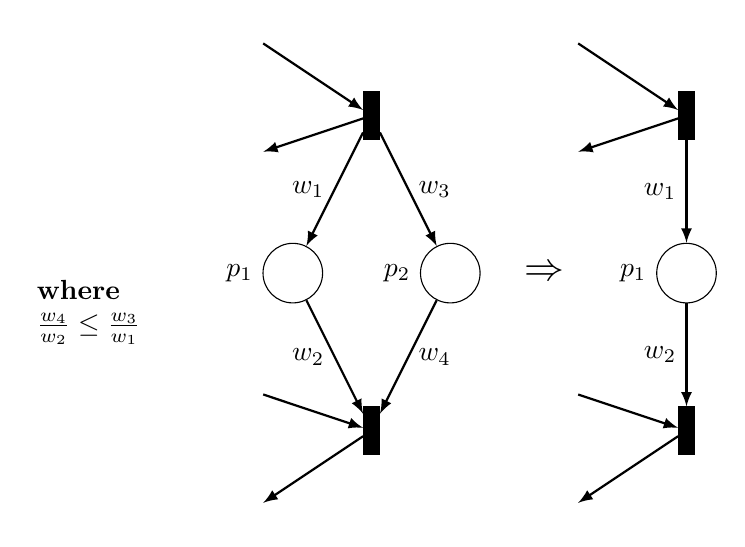
\begin{tikzpicture}
        %%% Before
        \begin{scope}
            % Places
            \node[place, label=left:$p_1$] (place1) at (-1,0) {};
            \node[place, label=left:$p_2$] (place2) at (1,0) {};

            % Transitions
            \node[transition,minimum height=6mm,minimum width=2mm,fill=black] (lTrans1) at (0,2) {};
            \node[transition,minimum height=6mm,minimum width=2mm,fill=black] (lTrans2) at (0,-2) {};

            % Invisible nodes
            \node (negIn1) at (-1.5,3) {};
            \node (negOut1) at (-1.5,1.5) {};
            \node (remIn1) at (-1.5,-1.5) {};
            \node (remOut1) at (-1.5,-3) {};

            % Arcs between transitions and places
            \draw[-latex,thick] (lTrans1) to node[left] {$w_1$} (place1);
            \draw[-latex,thick] (lTrans1) to node[right] {$w_3$} (place2);
            \draw[-latex,thick] (place1) to node[left] {$w_2$} (lTrans2);
            \draw[-latex,thick] (place2) to node[right] {$w_4$} (lTrans2);

            % Arcs to/from invisible nodes
            \draw[-latex,thick] (negIn1) -- node[above] {} (lTrans1);
            \draw[-latex,thick]  (remIn1) -- node[below] {} (lTrans2);
            \draw[-latex,thick]  (lTrans2) -- node[below] {} (remOut1);
            \draw[-latex,thick]  (lTrans1) -- node[above] {} (negOut1);
        \end{scope}

        \node (arrow) at (2.2,0) {\Large$\Rightarrow$};
        \node[text width=3.5cm] at (-2.5,-0.5) {\textbf{where }\\$\frac{w_4}{w_2}\leq\frac{w_3}{w_1}$};

        \begin{scope}
            % Places
            \node[place, label=left:$p_1$] (rplace1) at (4,0) {};

            % Transitions
            \node[transition,minimum height=6mm,minimum width=2mm,fill=black] (rTrans1) at (4,2) {};
            \node[transition,minimum height=6mm,minimum width=2mm,fill=black] (rTrans2) at (4,-2) {};

            % Arcs between transitions and places
            \draw[-latex,thick] (rTrans1) to node[left] {$w_1$} (rplace1);
            \draw[-latex,thick] (rplace1) to node[left] {$w_2$} (rTrans2);

            % Invisible nodes
            \node (rnegIn1) at (2.5,3) {};
            \node (rnegOut1) at (2.5,1.5) {};
            \node (rremIn1) at (2.5,-1.5) {};
            \node (rremOut1) at (2.5,-3) {};

            % Arcs to/from invisible nodes
            \draw[-latex,thick] (rnegIn1) -- node[above] {} (rTrans1);
            \draw[-latex,thick]  (rremIn1) -- node[below] {} (rTrans2);
            \draw[-latex,thick]  (rTrans2) -- node[below] {} (rremOut1);
            \draw[-latex,thick]  (rTrans1) -- node[above] {} (rnegOut1);
        \end{scope}
    \end{tikzpicture}
    \vspace{5mm}
    \begin{adjustbox}{center}
        \begin{tabular}{|p{65mm}|p{45mm}|} \hline
        Precondition & Update \\ \hline
        Fix places $p_1$ and $p_2$ s.t.:
        \begin{itemize}[leftmargin=10mm]
            \item[C1)] $p_2\notin places(\varphi)$
            \item[C2)] $p_2^\circ=\emptyset$
            \item[C3)] $p_1^\bullet\neq\emptyset$
            \item[C4)] $p_1^\bullet\supseteq p_2^\bullet$
            \item[C5)] ${}^\bullet p_1\subseteq{}^\bullet p_2$
            \item[C6)] $M(p_2) \geq M(p_1)\cdot d$
            \item[C7)] $d \leq f$
        \end{itemize}
        where
        \[
            d = \max_{t\in p_1^\bullet}\frac{\boxminus(p_2, t)}{\boxminus(p_1, t)}
        \]
        \[
            f = \min_{t\in{}^\bullet p_1}\frac{\boxplus(t, p_2)}{\boxplus(t, p_1)}
        \]
        &
        \begin{itemize}[leftmargin=10mm]
            \item[UC1)] Remove $p_2$
        \end{itemize} \\ \hline
        \end{tabular}
    \end{adjustbox}
    \caption{Rule C: Parallel places}
    \label{fig:rule_c}
\end{figure}

\begin{theorem}
    Rule~C shown in Figure~\ref{fig:rule_c} are correct for CTL* cardinality properties.
\end{theorem}

    \clearpage
    \section*{Rule E: Dead transition removal (P/T)}\label{sec:rule_e}
If a transition is initially not enabled due to a lack of tokens in $p_0$ and if $p_0$ is not able to gain tokens,
then the transition is dead and can be removed.
See Figure~\ref{fig:rule_e}.

\begin{theorem}\label{theorem:rule_e}
    Rule~E in Figure~\ref{fig:rule_e} is correct for CTL* cardinality properties.
\end{theorem}

\begin{figure}[h!]
    \centering
    \begin{tikzpicture}[scale=1.1]
        %%%% Before =====================================
        \begin{scope}
            % Places
            \node[place,label=right:$p_0$] (p0) at (0, -1) {$<w$};

            % Transitions
            \node[transition,fill=black,label=right:$t_0$] (t0) at (0, 1) {};

            % Invisible places
            \node (t0pre1) at (-.75, 2) {};
            \node (t0pre2) at (.75, 2) {};
            \node (t0post1) at (-1, 1.4) {};
            \node (t0post2) at (-1, .6) {};

            % Invisible transitions
            \node (p0pre1) at (-1, -0.5);
            \node (p0pre2) at (1, -0.5);
            \node (p0post1) at (-.75, -2);
            \node (p0post2) at (.75, -2);

            % Arcs
            \draw[-latex,thick] (t0pre1) -- (t0);
            \draw[-latex,thick] (t0pre2) -- (t0);
            \draw[-latex,thick] (t0) -- (t0post1);
            \draw[-latex,thick] (t0) -- (t0post2);
            \draw[-latex,thick] (t0) edge[bend right] (p0);
            \draw[-latex,thick] (p0) edge[bend right] node[right] {$w$} (t0);
            \draw[-latex,thick] (p0pre1) -- (p0);
            \draw[-latex,thick] (p0pre2) -- (p0);
            \draw[-latex,thick] (p0) -- (p0post1);
            \draw[-latex,thick] (p0) -- (p0post2);
        \end{scope}

        %%%% Arrow and conditions =======================
        \node (arrow) at (3,0) {\huge$\Rightarrow$};

        %%%% After ======================================
        \begin{scope}[shift={(6,1)},scale=1.1]
            % Places
            \node[place,label=right:$p_0$] (p0) at (0, -1) {$<w$};

            % Invisible transitions
            \node (p0pre1) at (-1, -0.5);
            \node (p0pre2) at (1, -0.5);
            \node (p0post1) at (-.75, -2);
            \node (p0post2) at (.75, -2);

            % Arcs
            \draw[-latex,thick] (p0pre1) -- (p0);
            \draw[-latex,thick] (p0pre2) -- (p0);
            \draw[-latex,thick] (p0) -- (p0post1);
            \draw[-latex,thick] (p0) -- (p0post2);
        \end{scope}
    \end{tikzpicture}
    \vspace{5mm}

    \begin{adjustbox}{center}
        \begin{tabular}{|p{79mm}|p{54mm}|} \hline
        Precondition & Update \\ \hline
        Fix place $p_0$ and transition $t_0$ s.t.:
        \begin{itemize}[leftmargin=10mm]
            \item[E1)] $M_0(p_0)<\boxminus(p_0, t_0)$
            \item[E2)] $\boxplus(t,p_0)\leq\boxminus(p_0, t)$ or $M_0(p_0)<\boxminus(p_0, t)$ for all $t\in T$
        \end{itemize} &
        \begin{itemize}[leftmargin=10mm]
            \item[UE1)] If $p_0^\bullet=\{t_0\},p_0^\circ=\emptyset$, and $p_0\notin places(\varphi)$ then remove $p_0$.
            \item[UE2)] Remove $t_0$
        \end{itemize} \\ \hline
        \end{tabular}
    \end{adjustbox}
    \caption{Rule E: Dead transition removal}
    \label{fig:rule_e}
\end{figure}
    \clearpage
    \section*{Rule F: Redundant place removal (P/T)}\label{sec:rule_f}
Rule~F defined in Figure~\ref{fig:rule_f} removes places which never inhibits any transitions.
This is done by check the minimum number of tokens added to the given place and its initial marking.

\begin{theorem}\label{theorem:rule_f}
    Rule~F in Figure~\ref{fig:rule_f} is correct for CTL*.
\end{theorem}

\begin{figure}[h!]
    \centering
    \begin{tikzpicture}[scale=1.1]
        %%%% Before =====================================
        \begin{scope}
            % Places
            \node[place,label=right:$p_0$] (p0) at (0, -1) {$\geq w$};

            % Transitions
            \node[transition,fill=black,label=right:$t$] (t0) at (0, 1) {};

            % Invisible places
            \node (t0pre1) at (-.75, 2) {};
            \node (t0pre2) at (.75, 2) {};
            \node (t0post1) at (-1, 1.4) {};
            \node (t0post2) at (-1, .6) {};

            % Invisible transitions
            \node (p0pre1) at (-1, -0.5);
            \node (p0pre2) at (1, -0.5);
            \node (p0post1) at (-.75, -2);
            \node (p0post2) at (.75, -2);

            % Arcs
            \draw[-latex,thick] (t0pre1) -- (t0);
            \draw[-latex,thick] (t0pre2) -- (t0);
            \draw[-latex,thick] (t0) -- (t0post1);
            \draw[-latex,thick] (t0) -- (t0post2);
            \draw[-latex,thick] (t0) edge[bend right] node[left] {$\geq w$} (p0);
            \draw[-latex,thick] (p0) edge[bend right] node[right] {$w$} (t0);
            \draw[-latex,thick] (p0pre1) -- (p0);
            \draw[-latex,thick] (p0pre2) -- (p0);
            \draw[-latex,thick] (p0) -- (p0post1);
            \draw[-latex,thick] (p0) -- (p0post2);
        \end{scope}

        %%%% Arrow and conditions =======================
        \node (arrow) at (3,0) {\huge$\Rightarrow$};

        %%%% After ======================================
        \begin{scope}[shift={(6,-1)},scale=1.1]
            % Transitions
            \node[transition,fill=black,label=right:$t$] (t0) at (0, 1) {};

            % Invisible places
            \node (t0pre1) at (-.75, 2) {};
            \node (t0pre2) at (.75, 2) {};
            \node (t0post1) at (-1, 1.4) {};
            \node (t0post2) at (-1, .6) {};

            % Arcs
            \draw[-latex,thick] (t0pre1) -- (t0);
            \draw[-latex,thick] (t0pre2) -- (t0);
            \draw[-latex,thick] (t0) -- (t0post1);
            \draw[-latex,thick] (t0) -- (t0post2);
        \end{scope}
    \end{tikzpicture}
    \vspace{5mm}

    \begin{adjustbox}{center}
        \begin{tabular}{|p{79mm}|p{54mm}|} \hline
        Precondition & Update \\ \hline
        Fix place $p_0$ s.t.:
        \begin{itemize}[leftmargin=10mm]
            \item[F1)] $p_0^\circ=\emptyset$ and $p_0\notin places(\varphi)$
            \item[F2)] $\boxplus(t, p_0)\geq\boxminus(p_0, t)$ and $M_0(p_0)\geq\boxminus(p_0, t)$ for all $t\in T$
        \end{itemize} &
        \begin{itemize}[leftmargin=10mm]
            \item[UF1)] Remove $p_0$
        \end{itemize} \\ \hline
        \end{tabular}
    \end{adjustbox}
    \caption{Rule F: Redundant place removal}
    \label{fig:rule_f}
\end{figure}

    \clearpage
    \section*{Rule I: Irrelevant Net Sections}
Rule~I removes places and transitions that cannot affect reachability.
It marks places and transitions that appear in the query and their direct consumers as relevant, and then iteratively
propagates this relevance to all pre sets of relevant places and transitions, and removes everything that does not end
up being relevant at the end. \\
Figure~\ref{fig:rule_i} shows an example where the query mentions none of the shown net, but does mention a place that $t_3$ can affect.

\begin{figure}[h]
    \centering
    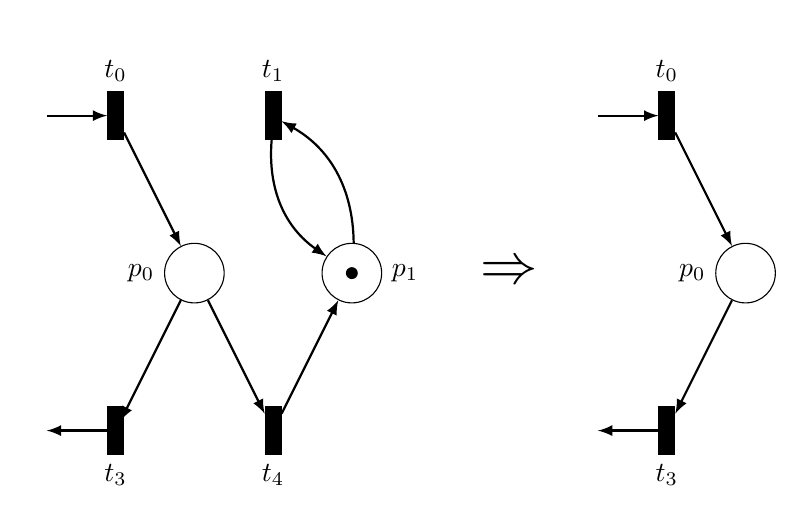
\begin{tikzpicture}
        % Left side places
        \node[place,label=left:$p_0$] (place1) at (0,0) {};
        \node[place,label=right:$p_1$, tokens=1] (place2) at (2,0) {};

        % Left side transition
        \node[transition,minimum height=6mm,minimum width=2mm,fill=black,label=above:$t_0$] (negTrans1) at (-1,2) {};
        \node[transition,minimum height=6mm,minimum width=2mm,fill=black,label=above:$t_1$] (remTrans1) at (1,2) {};
        \node[transition,minimum height=6mm,minimum width=2mm,fill=black,label=below:$t_4$] (trans3) at (1,-2) {};
        \node[transition,minimum height=6mm,minimum width=2mm,fill=black,label=below:$t_3$] (trans4) at (-1,-2) {};

        % Left side invisible nodes
        \node (negIn1) at (-2,2) {};
        \node (negOut1) at (1,3) {};
        \node (placeIn1) at (-1,-2) {};
        %\node (remIn1) at (1,-1) {};
        %\node (remOut1) at (1,-3) {};
        \node (out4) at (-2,-2) {};

        % Left side arcs between transitions and nodes
        \draw[-latex,thick] (negTrans1) edge node[left] {} (place1);
        %\draw[-latex,thick] (place1) edge[bend right] node[right] {$w_3$} (negTrans1);
        %\draw[-latex,thick] (place1) edge[bend right] node[left] {$w_1$} (remTrans1);
        %\draw[-latex,thick] (remTrans1) edge node[right] {} (place1);

        % Left side arcs to/from invisible nodes
        \draw[-latex,thick] (negIn1) -- (negTrans1);
        %\draw[-latex,thick] (negTrans1) -- (negOut1);
        \draw[-latex,thick] (place1) -- (placeIn1);
        \draw[-latex,thick] (trans3) -- (place2);
        \draw[-latex,thick] (remTrans1) edge[bend right] node[right] {} (place2);
        \draw[-latex,thick] (place2) edge[bend right] node[below left] {} (remTrans1);
        \draw[-latex,thick] (place1) -- (trans3);
        \draw[-latex,thick] (trans4) -- (out4);

        % ================== Middle arrow ==================
        \node (arrow) at (4,0) {\huge$\Rightarrow$};
        %\node[text width=3.5cm] at (4, -2) {\textbf{where}\\$places(\varphi) = \{p_0\}$};

        % ==================================================

        % Left side places
        \node[place,label=left:$p_0$] (rplace1) at (7,0) {};
        %\node[place,label=right:$p_1$] (place2) at (8,0) {$\neg \varphi$};

        % Left side transition
        \node[transition,minimum height=6mm,minimum width=2mm,fill=black,label=above:$t_0$] (rnegTrans1) at (6,2) {};
        %\node[transition,minimum height=6mm,minimum width=2mm,fill=black,label=above:$t_1$] (rremTrans1) at (8,2) {};
        \node[transition,minimum height=6mm,minimum width=2mm,fill=black,label=below:$t_3$] (rtrans4) at (6,-2) {};

        % Left side invisible nodes
        \node (rnegIn1) at (5,2) {};
        \node (rnegOut1) at (6,3) {};
        %\node (rplaceIn1) at (5,0) {};
        %\node (remIn1) at (1,-1) {};
        %\node (remOut1) at (1,-3) {};
        \node (rout4) at (5,-2) {};

        % Left side arcs between transitions and nodes
        \draw[-latex,thick] (rnegTrans1) edge node[left] {} (rplace1);
        %\draw[-latex,thick] (place1) edge[bend right] node[right] {$w_3$} (negTrans1);
        %\draw[-latex,thick] (place1) edge[bend right] node[left] {$w_1$} (remTrans1);
        %\draw[-latex,thick] (rremTrans1) edge node[right] {} (rplace1);

        % Left side arcs to/from invisible nodes
        \draw[-latex,thick] (rnegIn1) -- (rnegTrans1);
        %\draw[-latex,thick] (negTrans1) -- (negOut1);
        \draw[-latex,thick] (rplace1) -- (rtrans4);
        %\draw[-latex,thick] (place2) -- (trans3);
        %\draw[-latex,thick] (remTrans1) -- (place2);
        \draw[-latex,thick] (rtrans4) -- (rout4);
    \end{tikzpicture}
    \caption{Rule I: Irrelevant net sections}
    \label{fig:rule_i}
\end{figure}
    \clearpage
    \section*{Rule L: Dominated Transition (P/T)}\label{sec:rule_l}
Rule L removes transitions that have the same effect as another transition, but with more preconditions.
Since both transitions lead to the same state, we can therefore remove the one
with the higher preconditions and use the other instead.
See the formal description in Figure~\ref{fig:rule_l}.

\begin{figure}[h!]
    \centering
    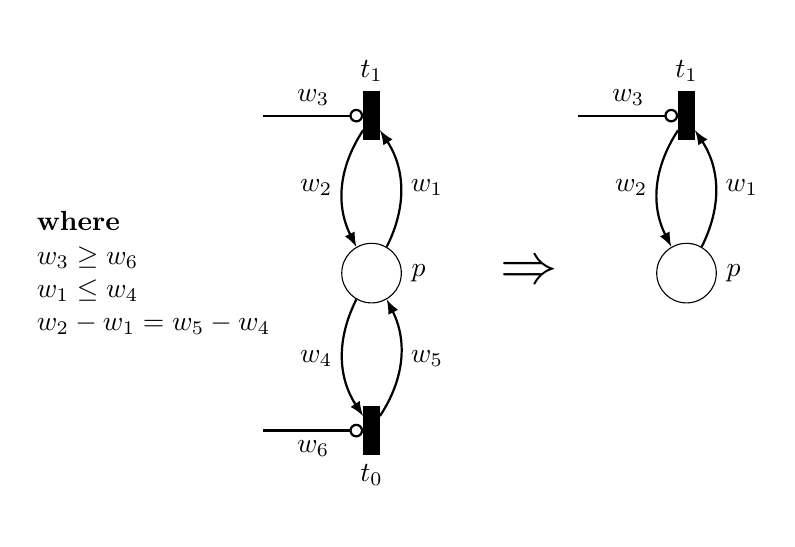
\begin{tikzpicture}
        % Left side places
        \node[place, label=right:$p$] (place1) at (0,0) {};

        % Left side transition
        \node[transition,minimum height=6mm,minimum width=2mm,fill=black,label=above:$t_1$] (lTrans1) at (0,2) {};
        \node[transition,minimum height=6mm,minimum width=2mm,fill=black,label=below:$t_0$] (lTrans2) at (0,-2) {};

        % Left side invisible nodes
        \node (negIn1) at (-1.5,2) {};
        \node (negOut1) at (1,3) {};
        \node (remIn1) at (-1.5,-2) {};
        \node (remOut1) at (1,-3) {};

        % Left side arcs between transitions and nodes
        \draw[-latex,thick] (lTrans1) edge[bend right] node[left] {$w_2$} (place1);
        \draw[-latex,thick] (place1) edge[bend right] node[right] {$w_1$} (lTrans1);
        \draw[-latex,thick] (lTrans2) edge[bend right] node[right] {$w_5$} (place1);
        \draw[-latex,thick] (place1) edge[bend right] node[left] {$w_4$} (lTrans2);

        % Left side arcs to/from invisible nodes
        \draw[-{Circle[open]},thick] (negIn1) -- node[above] {$w_3$} (lTrans1);
        \draw[-{Circle[open]},thick]  (remIn1) -- node[below] {$w_6$} (lTrans2);

        % ================== Middle arrow ==================
        \node (arrow) at (2,0) {\huge$\Rightarrow$};
        \node[text width=3.5cm] at (-2.5,0) {\textbf{where }\\$w_3\geq w_6$\\$w_1\leq w_4$\\$w_2-w_1= w_5-w_4$};
        % ==================================================

        % Right side places
        \node[place, label=right:$p$] (place2) at (4,0) {};

        % Right side transitions
        \node[transition,minimum height=6mm,minimum width=2mm,fill=black,label=above:$t_1$] (rTrans1) at (4,2) {};

        % Right side invisible nodes
        \node (negIn2) at (2.5,2) {};

        % Right side arcs between places and transition
        \draw[-latex,thick] (rTrans1) edge[bend right] node[left] {$w_2$} (place2);
        \draw[-latex,thick] (place2) edge[bend right] node[right] {$w_1$} (rTrans1);

        \draw[-{Circle[open]},thick]  (negIn2) -- node[above] {$w_3$} (rTrans1);


    \end{tikzpicture}
    \vspace{5mm}
    \begin{adjustbox}{center}
        \begin{tabular}{|p{55mm}|p{45mm}|} \hline
        Precondition & Update \\ \hline
        Fix transition $t_1$ and $t_0$ s.t.:
        \begin{itemize}[leftmargin=10mm]
            \item[L1)] $I(t_1)\geq I(t_0)$
            \item[L2)] $\boxminus(t_1)\leq \boxminus(t_0)$
            \item[L3)] $E(t_1)=E(t_0)$
        \end{itemize}
        &
        \begin{itemize}[leftmargin=10mm]
            \item[UL1)] Remove $t_0$
        \end{itemize} \\ \hline
        \end{tabular}
    \end{adjustbox}
    \caption{Rule L: Dominated Transition}
    \label{fig:rule_l}
\end{figure}

\begin{theorem}
    Rule~L in Figure~\ref{fig:rule_l} is correct for CTL* cardinality properties.
\end{theorem}

    \clearpage
    \section*{Rule M: Effectively dead places and transitions}\label{sec:rule_m}
The Rule~M finds and removes effectively dead places and transitions.
We define an effectively dead place to be a place that will never gain nor lose tokens.
Effectively dead transitions are transitions that are initially disabled (and/or inhibited)
by a place that cannot gain (and/or lose) tokens.
These places and transitions are found using fixed-point iteration as defined in Algorithm~\ref{algo:rule_m}.

\begin{algorithm}
    \vspace{0.2cm}
    \caption{Rule M: Effectively dead places and transitions}
    \label{algo:rule_m}
    \DontPrintSemicolon
    \LinesNumbered
    \KwIn{A net $N=\langle P,T,\boxminus,\boxplus,I \rangle$, initial marking $M_0$ and CTL* formula $\varphi$}
    \KwOut{A reduced net $N'$ and its initial marking $M_0'$}
    \vspace{1mm}
    $S_\leq:=P$\tcc*{Places that cannot gain tokens}
    $S_\geq:=P$\tcc*{Places that cannot lose tokens}
    $F:=T$\tcc*{Transitions that cannot fire}
    \Do{$S_\leq$, $S_\geq$, and $F$ do not change}{
        \tcc*{Find transitions that may fire and update sets accordingly}
        \ForEach{$t\in F$ where $\forall p\in P.(\boxminus(p,t)\leq M_0(p)\lor p\notin S_\leq)\land(I(p,t)>M_0(p)\lor p\notin S_\geq)$}{
            $F:=F\setminus\{t\}$\;
            $S_\leq:=S_\leq\setminus t^\boxplus$\;
            $S_\geq:=S_\geq\setminus {}^\boxminus t$\;
        }
    }
    $P':=P\setminus(S_\leq\cap S_\geq\setminus places(\varphi))$\;
    $T':=T\setminus F$\;
    \KwRet{$N'=\langle P', T', \boxminus, \boxplus, I\rangle$ and $M_0$}
    \vspace{0.2cm}
\end{algorithm}

\begin{theorem}\label{theorem:rule_m}
    Rule~M in Algorithm~\ref{algo:rule_m} is correct for CTL* cardinality properties.
\end{theorem}
\begin{theorem}\label{theorem:rule_m_supercedes_e}
Rule~M supercedes Rule~E.
\end{theorem}

    \clearpage
    \section*{Rule N: Redundant arc removal}\label{sec:rule_n}
The lower bound number of tokens at a place $p_0$ is given by the minimum of the initial marking
and the number of tokens returned by any consuming transition with a negative effect on $p_0$.
Using the lower bound we can then find transitions, which are never disabled by $p_0$ and
remove the transition's dependency on $p_0$, since it is unnecessary,
as long as we maintain the effect of firing the transition.

\begin{figure}[h!]
    \centering
    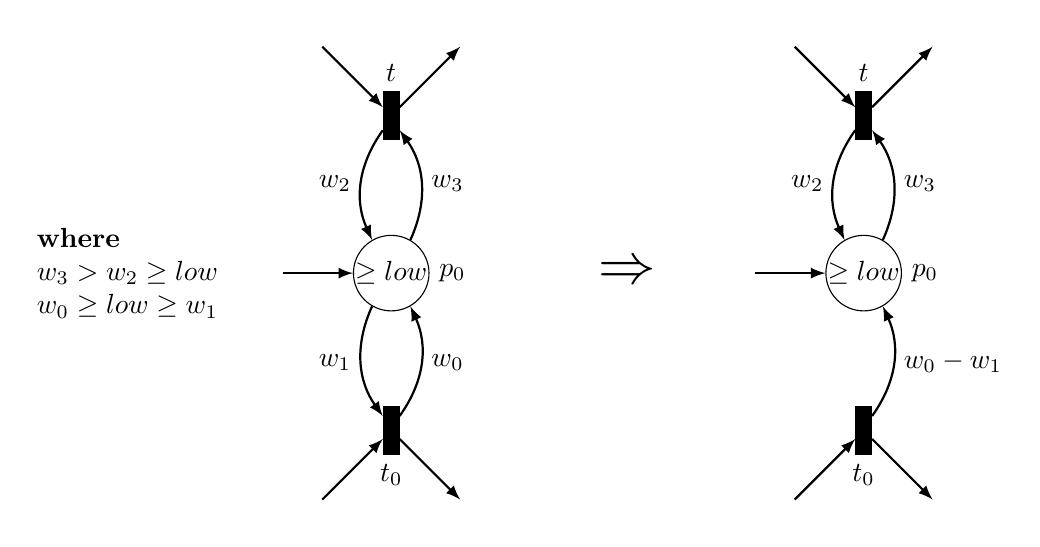
\begin{tikzpicture}
        % Left side places
        \node[place,label=right:$p_0$] (place1) at (0,0) {$\geq low$};

        % Left side transition
        \node[transition,minimum height=6mm,minimum width=2mm,fill=black,label=above:$t$] (negTrans1) at (0,2) {};
        \node[transition,minimum height=6mm,minimum width=2mm,fill=black,label=below:$t_0$] (remTrans1) at (0,-2) {};

        % Left side invisible nodes
        \node (negIn1) at (-1,3) {};
        \node (negOut1) at (1,3) {};
        \node (placeIn1) at (-1.5,0) {};
        \node (remIn1) at (-1,-3) {};
        \node (remOut1) at (1,-3) {};

        % Left side arcs between transitions and nodes
        \draw[-latex,thick] (negTrans1) edge[bend right] node[left] {$w_2$} (place1);
        \draw[-latex,thick] (place1) edge[bend right] node[right] {$w_3$} (negTrans1);
        \draw[-latex,thick] (place1) edge[bend right] node[left] {$w_1$} (remTrans1);
        \draw[-latex,thick] (remTrans1) edge[bend right] node[right] {$w_0$} (place1);

        % Left side arcs to/from invisible nodes
        \draw[-latex,thick] (negIn1) -- (negTrans1);
        \draw[-latex,thick] (negTrans1) -- (negOut1);
        \draw[-latex,thick] (placeIn1) -- (place1);
        \draw[-latex,thick] (remIn1) -- (remTrans1);
        \draw[-latex,thick] (remTrans1) -- (remOut1);

        % ================== Middle arrow ==================
        \node (arrow) at (3,0) {\huge$\Rightarrow$};
        \node[text width=3cm] at (-3, 0) {\textbf{where}\\$w_3>w_2\geq low$\\$w_0 \geq low \geq w_1$};
        % ==================================================

        % Right side places
        \node[place,label=right:$p_0$] (place2) at (6,0) {$\geq low$};

        % Right side transitions
        \node[transition,minimum height=6mm,minimum width=2mm,fill=black,label=above:$t$] (negTrans2) at (6,2) {};
        \node[transition,minimum height=6mm,minimum width=2mm,fill=black,label=below:$t_0$] (remTrans2) at (6,-2) {};

        % Right side invisible nodes
        \node (negIn2) at (5,3) {};
        \node (negOut2) at (7,3) {};
        \node (placeIn2) at (4.5,0) {};
        \node (remIn2) at (5,-3) {};
        \node (remOut2) at (7,-3) {};

        % Right side arcs between places and transition
        \draw[-latex,thick] (negTrans2) edge[bend right] node[left] {$w_2$} (place2);
        \draw[-latex,thick] (place2) edge[bend right] node[right] {$w_3$} (negTrans2);
        \draw[-latex,thick] (remTrans2) edge[bend right] node[right] {$w_0-w_1$} (place2);

        % Right side arcs to/from invisible nodes
        \draw[-latex,thick] (negIn2) -- (negTrans2);
        \draw[-latex,thick] (negTrans2) -- (negOut2);
        \draw[-latex,thick] (placeIn2) -- (place2);
        \draw[-latex,thick] (remIn2) -- (remTrans2);
        \draw[-latex,thick] (remTrans2) -- (remOut2);

    \end{tikzpicture}
    \vspace{1cm}

    \begin{adjustbox}{center}
        \begin{tabular}{|p{70mm}|p{75mm}|} \hline
        Precondition & Update \\ \hline
        Fix place $p_0$ and transition $t_0$ s.t.:
        \begin{itemize}[leftmargin=10mm]
            \item[N1)] $t_0\in p_0^\bullet\setminus p_0^\boxminus$
            \item[N2)] $\boxminus(p_0,t_0)\leq low$
        \end{itemize}
        where
        \begin{itemize}
            \item[] $low=\min\{M_0(p_0)\}\cup\{\boxplus(p_0, t)\mid t\in p_0^\boxminus\}$
        \end{itemize} &
        \begin{itemize}[leftmargin=10mm]
            \item[UN1)] Set $\boxplus(p_0,t_0):=\boxplus(p_0,t_0)-\boxminus(p_0,t_0)$
            \item[UN2)] Set $\boxminus(p_0,t_0):=0$
        \end{itemize} \\ \hline
        \end{tabular}
    \end{adjustbox}
    \caption{Rule N: Redundant arc removal}
    \label{fig:rule_n}
\end{figure}

\begin{theorem}\label{theorem:rule_n}
    Rule~N in Figure~\ref{fig:rule_n} is correct for CTL*.
\end{theorem}
    \clearpage
    \section*{Rule O: Inhibited transition}\label{sec:rule_o}
We can find the lower bound of tokens at a place $p_0$.
Any inhibitor arc from $p_0$ with a weight smaller than the lower bound
always inhibits the given transition, which means that the transition can be removed.
See Figure~\ref{fig:rule_o} for a formal description of Rule~O.

\begin{figure}[h!]
    \centering
    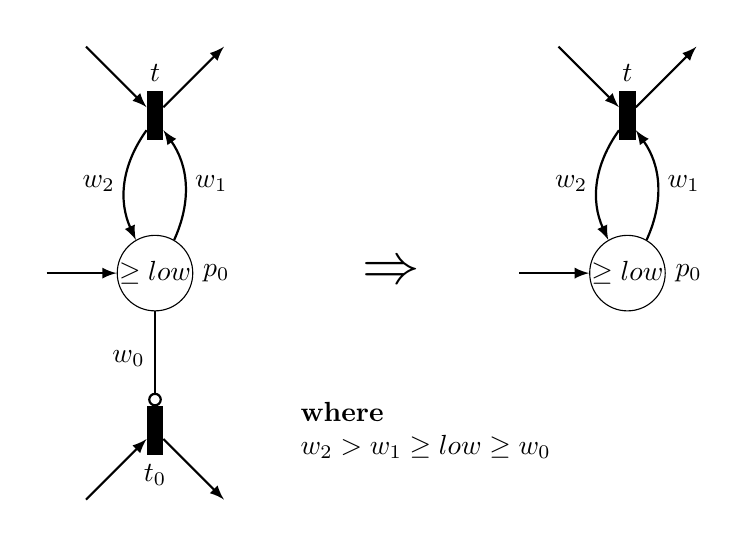
\begin{tikzpicture}
        % Left side places
        \node[place,label=right:$p_0$] (place1) at (0,0) {$\geq low$};

        % Left side transition
        \node[transition,minimum height=6mm,minimum width=2mm,fill=black,label=above:$t$] (negTrans1) at (0,2) {};
        \node[transition,minimum height=6mm,minimum width=2mm,fill=black,label=below:$t_0$] (remTrans1) at (0,-2) {};

        % Left side invisible nodes
        \node (negIn1) at (-1,3) {};
        \node (negOut1) at (1,3) {};
        \node (placeIn1) at (-1.5,0) {};
        \node (remIn1) at (-1,-3) {};
        \node (remOut1) at (1,-3) {};

        % Left side arcs between transitions and nodes
        \draw[-latex,thick] (negTrans1) edge[bend right] node[left] {$w_2$} (place1);
        \draw[-latex,thick] (place1) edge[bend right] node[right] {$w_1$} (negTrans1);
        \draw[-{Circle[open]},thick] (place1) -- node[left] {$w_0$} (remTrans1);

        % Left side arcs to/from invisible nodes
        \draw[-latex,thick] (negIn1) -- (negTrans1);
        \draw[-latex,thick] (negTrans1) -- (negOut1);
        \draw[-latex,thick] (placeIn1) -- (place1);
        \draw[-latex,thick] (remIn1) -- (remTrans1);
        \draw[-latex,thick] (remTrans1) -- (remOut1);

        % ================== Middle arrow ==================
        \node (arrow) at (3,0) {\huge$\Rightarrow$};
        \node[text width=3.5cm] at (3.6, -2) {\textbf{where}\\$w_2>w_1\geq low\geq w_0$};
        % ==================================================

        % Right side places
        \node[place,label=right:$p_0$] (place2) at (6,0) {$\geq low$};

        % Right side transitions
        \node[transition,minimum height=6mm,minimum width=2mm,fill=black,label=above:$t$] (negTrans2) at (6,2) {};

        % Right side invisible nodes
        \node (negIn2) at (5,3) {};
        \node (negOut2) at (7,3) {};
        \node (placeIn2) at (4.5,0) {};

        % Right side arcs between places and transition
        \draw[-latex,thick] (negTrans2) edge[bend right] node[left] {$w_2$} (place2);
        \draw[-latex,thick] (place2) edge[bend right] node[right] {$w_1$} (negTrans2);

        % Right side arcs to/from invisible nodes
        \draw[-latex,thick] (negIn2) -- (negTrans2);
        \draw[-latex,thick] (negTrans2) -- (negOut2);
        \draw[-latex,thick] (placeIn2) -- (place2);

    \end{tikzpicture}
    \vspace{1cm}

    \begin{adjustbox}{center}
        \begin{tabular}{|p{80mm}|p{45mm}|} \hline
        Precondition & Update \\ \hline
        Fix place $p_0$ and transition $t_0$ s.t.:
        \begin{itemize}[leftmargin=10mm]
            \item[O1)] $t_0\in p_0^\circ$
            \item[O2)] $I(p_0,t_0)\leq low$
        \end{itemize}
        where
        \[
            low=\min\{M_0(p_0)\}\cup\{\boxplus(p_0, t)\mid t\in p_0^\boxminus\}
        \]
        &
        \begin{itemize}[leftmargin=10mm]
            \item[UO1)] Remove $t_0$.
        \end{itemize} \\ \hline
        \end{tabular}
    \end{adjustbox}
    \caption{Rule O: Inhibited transition}
    \label{fig:rule_o}
\end{figure}

\begin{theorem}
    Rule~O in Figure~\ref{fig:rule_o} is correct for CTL* cardinality properties.
\end{theorem}

    \clearpage
    % Preamble
\documentclass[11pt]{article}

% Packages
\usepackage{amsmath}
\usepackage{amssymb}
\usepackage{tikz}
\usetikzlibrary{arrows,arrows.meta,positioning,calc,petri}
\usepackage{adjustbox}
\usepackage{enumitem}
\usepackage{listings}
\usepackage[ruled,vlined]{algorithm2e}
\SetKwRepeat{Do}{do}{until}%
\newtheorem{theorem}{Theorem}

% Document
\begin{document}

    \section*{Rule P: Redundant inhibitor arc}\label{sec:rule_p}
    Sometimes we can find an upper bound on the number of tokens at a place $p_0$.
    This upper bound is given by the initial marking if all transitions have a non-positive effect on $p_0$.
    Any inhibitor arc from $p_0$ with a weight higher than the upper bound of $p_0$ therefore never inhibits,
    which means the inhibitor arc can be removed.
    See Figure~\ref{fig:rule_p} for a formal description of Rule~P.

    \begin{figure}[h!]
        \centering
        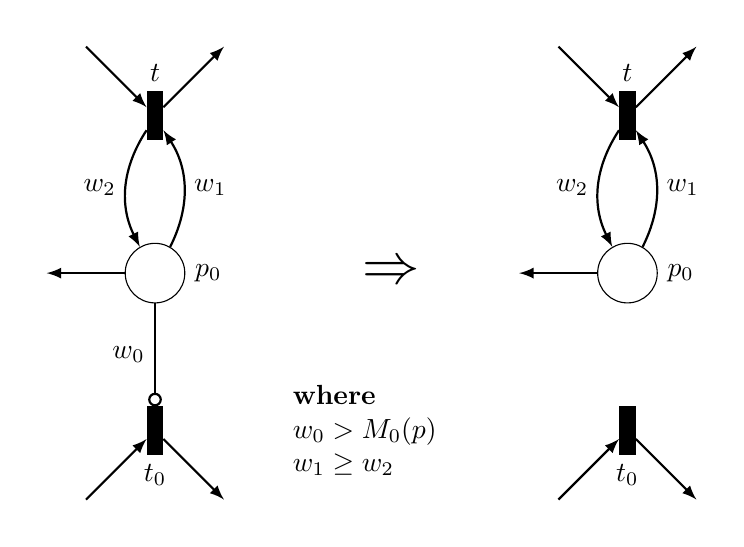
\begin{tikzpicture}
            % Left side places
            \node[place,label=right:$p_0$] (place1) at (0,0) {};

            % Left side transition
            \node[transition,minimum height=6mm,minimum width=2mm,fill=black,label=above:$t$] (negTrans1) at (0,2) {};
            \node[transition,minimum height=6mm,minimum width=2mm,fill=black,label=below:$t_0$] (remTrans1) at (0,-2) {};

            % Left side invisible nodes
            \node (negIn1) at (-1,3) {};
            \node (negOut1) at (1,3) {};
            \node (placeIn1) at (-1.5,0) {};
            \node (remIn1) at (-1,-3) {};
            \node (remOut1) at (1,-3) {};

            % Left side arcs between transitions and nodes
            \draw[-latex,thick] (negTrans1) edge[bend right] node[left] {$w_2$} (place1);
            \draw[-latex,thick] (place1) edge[bend right] node[right] {$w_1$} (negTrans1);
            \draw[-{Circle[open]},thick] (place1) -- node[left] {$w_0$} (remTrans1);

            % Left side arcs to/from invisible nodes
            \draw[-latex,thick] (negIn1) -- (negTrans1);
            \draw[-latex,thick] (negTrans1) -- (negOut1);
            \draw[-latex,thick] (place1) -- (placeIn1);
            \draw[-latex,thick] (remIn1) -- (remTrans1);
            \draw[-latex,thick] (remTrans1) -- (remOut1);

            % ================== Middle arrow ==================
            \node (arrow) at (3,0) {\huge$\Rightarrow$};
            \node[text width=3.5cm] at (3.5, -2) {\textbf{where}\\$w_0>M_0(p)$\\$w_1\geq w_2$};
            % ==================================================

            % Right side places
            \node[place,label=right:$p_0$] (place2) at (6,0) {};

            % Right side transitions
            \node[transition,minimum height=6mm,minimum width=2mm,fill=black,label=above:$t$] (rTrans2) at (6,2) {};
            \node[transition,minimum height=6mm,minimum width=2mm,fill=black,label=below:$t_0$] (rTrans1) at (6,-2) {};

            % Right side invisible nodes
            \node (invinrt2) at (5,3) {};
            \node (invoutrt2) at (7,3) {};
            \node (placeIn2) at (4.5,0) {};
            \node (invinrt1) at (5,-3) {};
            \node (invoutrt1) at (7,-3) {};

            % Right side arcs between places and transition
            \draw[-latex,thick] (rTrans2) edge[bend right] node[left] {$w_2$} (place2);
            \draw[-latex,thick] (place2) edge[bend right] node[right] {$w_1$} (rTrans2);

            % Right side arcs to/from invisible nodes
            \draw[-latex,thick] (invinrt2) -- (rTrans2);
            \draw[-latex,thick] (rTrans2) -- (invoutrt2);
            \draw[-latex,thick] (place2) -- (placeIn2);
            \draw[-latex,thick] (invinrt1) -- (rTrans1);
            \draw[-latex,thick] (rTrans1) -- (invoutrt1);

        \end{tikzpicture}
        \vspace{1cm}

        \begin{adjustbox}{center}
            \begin{tabular}{|p{65mm}|p{45mm}|} \hline
            Precondition & Update \\ \hline
            Fix place $p_0$ and transition $t_0$ s.t.:
            \begin{itemize}[leftmargin=10mm]
                \item[P1)] $t_0\in p_0^\circ$
                \item[P2)] $I(p_0,t_0)> M_0(p_0)$
                \item[P3)] $^\boxplus p_0 = \emptyset$
            \end{itemize}
            &
            \begin{itemize}[leftmargin=10mm]
                \item[UP1)] $I(p_0,t_0) = \infty$.
            \end{itemize} \\ \hline
            \end{tabular}
        \end{adjustbox}
        \caption{Rule P: Redundant inhibitor arc}
        \label{fig:rule_p}
    \end{figure}

    \begin{theorem}
        Rule~P in Figure~\ref{fig:rule_p} is correct for CTL*.
    \end{theorem}

\end{document}

    \clearpage
    \section*{Rule~Q: Preemptive transition firing}
Rule~Q evaluates transitions that are initially enabled and are the only consumer of all places in its pre set.
The formal description of Rule~Q can be found in Figure~\ref{fig:rule_q}.
Remark that Rule~Q can potentially put tokens into places which will prevent other reductions.
Furthermore, it can be applied infinitely if $\boxminus(t_0)\leq \boxplus(t_0)$, or if the Petri net contains a loop.

\begin{figure}[h!]
    \centering
    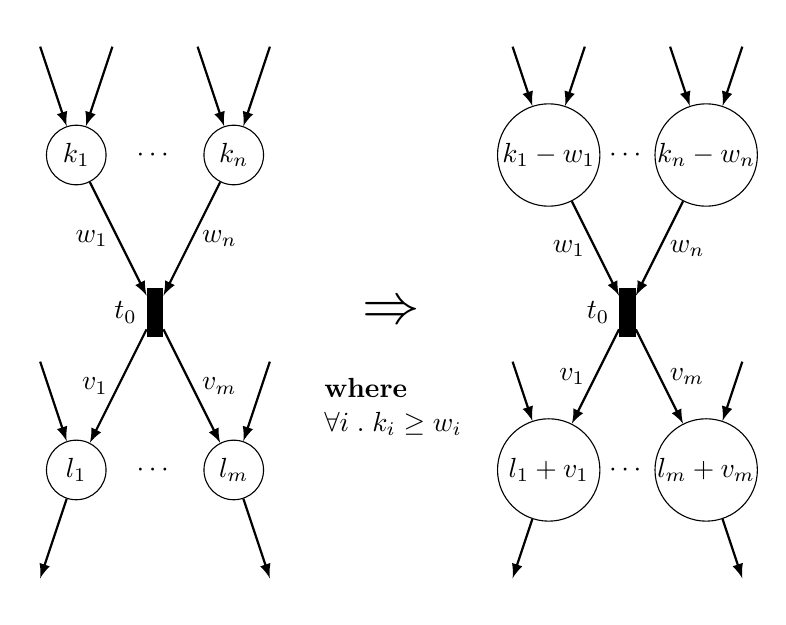
\begin{tikzpicture}
        % Left side places
        \node[place] (lplace1) at (0,2) {$k_1$};
        \node[place] (lplace2) at (2,2) {$k_n$};
        \node at (1,2) {$\cdots$};
        \node[place] (lplace3) at (0,-2) {$l_1$};
        \node[place] (lplace4) at (2,-2) {$l_m$};
        \node at (1,-2) {$\cdots$};

        % Left side transition
        \node[transition,minimum height=6mm,minimum width=2mm,fill=black,label=left:$t_0$] (ltrans) at (1,0) {};
        %\node[transition,minimum height=6mm,minimum width=2mm,fill=black,label=below:$t_0$] (remTrans1) at (0,-2) {};

        % Left side invisible nodes
        \node (lp1in1) at (-0.5,3.5) {};
        \node (lp1in2) at (0.5,3.5) {};
        \node (lp2in1) at (1.5,3.5) {};
        \node (lp2in2) at (2.5,3.5) {};
        \node (lp3in1) at (-0.5,-0.5) {};
        \node (lp4in1) at (2.5,-0.5) {};
        \node (lp3out1) at (-0.5,-3.5) {};
        \node (lp4out1) at (2.5,-3.5) {};

        % Left side arcs between transitions and nodes
        \draw[-latex,thick] (lplace1) edge node[left] {$w_1$} (ltrans);
        \draw[-latex,thick] (lplace2) edge node[right] {$w_n$} (ltrans);
        \draw[-latex,thick] (ltrans) edge node[left] {$v_1$} (lplace3);
        \draw[-latex,thick] (ltrans) edge node[right] {$v_m$} (lplace4);

        % Left side arcs to/from invisible nodes
        \draw[-latex,thick] (lp1in1) -- (lplace1);
        \draw[-latex,thick] (lp1in2) -- (lplace1);
        \draw[-latex,thick] (lp2in1) -- (lplace2);
        \draw[-latex,thick] (lp2in2) -- (lplace2);
        \draw[-latex,thick] (lp3in1) -- (lplace3);
        \draw[-latex,thick] (lp4in1) -- (lplace4);
        \draw[-latex,thick] (lplace3) -- (lp3out1);
        \draw[-latex,thick] (lplace4) -- (lp4out1);

        % ================== Middle arrow ==================
        \node (arrow) at (4,0) {\huge$\Rightarrow$};
        \node[text width=3.5cm] at (4.9, -1.2) {\textbf{where}\\$\forall i\;.\;k_i\geq w_i$};
        % ==================================================

        % Right side places
        \node[place,minimum size=1.3cm] (rplace1) at (6,2) {$k_1 - w_1$};
        \node at (7,2) {$\cdots$};
        \node[place,minimum size=1.3cm] (rplace2) at (8,2) {$k_n - w_n$};
        \node[place,minimum size=1.3cm] (rplace3) at (6,-2) {$l_1 + v_1$};
        \node at (7,-2) {$\cdots$};
        \node[place,minimum size=1.3cm] (rplace4) at (8,-2) {$l_m + v_m$};

        % Right side transition
        \node[transition,minimum height=6mm,minimum width=2mm,fill=black,label=left:$t_0$] (rtrans) at (7,0) {};
        %\node[transition,minimum height=6mm,minimum width=2mm,fill=black,label=below:$t_0$] (remTrans1) at (0,-2) {};

        % Right side invisible nodes
        \node (rp0in1) at (5.5,3.5) {};
        \node (rp0in2) at (6.5,3.5) {};
        \node (rp1in1) at (7.5,3.5) {};
        \node (rp1in2) at (8.5,3.5) {};
        \node (rp2in1) at (5.5,-0.5) {};
        \node (rp3in1) at (8.5,-0.5) {};
        \node (rp2out1) at (5.5,-3.5) {};
        \node (rp3out1) at (8.5,-3.5) {};

        % Right side arcs between transitions and nodes
        \draw[-latex,thick] (rplace1) edge node[left] {$w_1$} (rtrans);
        \draw[-latex,thick] (rplace2) edge node[right] {$w_n$} (rtrans);
        \draw[-latex,thick] (rtrans) edge node[left] {$v_1$} (rplace3);
        \draw[-latex,thick] (rtrans) edge node[right] {$v_m$} (rplace4);

        % Right side arcs to/from invisible nodes
        \draw[-latex,thick] (rp0in1) -- (rplace1);
        \draw[-latex,thick] (rp0in2) -- (rplace1);
        \draw[-latex,thick] (rp1in1) -- (rplace2);
        \draw[-latex,thick] (rp1in2) -- (rplace2);
        \draw[-latex,thick] (rp2in1) -- (rplace3);
        \draw[-latex,thick] (rp3in1) -- (rplace4);
        \draw[-latex,thick] (rplace3) -- (rp2out1);
        \draw[-latex,thick] (rplace4) -- (rp3out1);
    \end{tikzpicture}
    \vspace{1cm}

    \begin{adjustbox}{center}
        \begin{tabular}{|p{65mm}|p{45mm}|} \hline
        Precondition & Update \\ \hline
        Fix transition $t_0$ s.t.:
        \begin{itemize}[leftmargin=10mm]
            \item[Q1)] $({}^\bullet t)^\bullet = \{t_0\}$
            \item[Q2)] $\boxminus(t_0) \leq M_0 < I(t_0)$
            \item[Q3)] $({}^\bullet t_0 \cup t_0^\bullet) \cap
            places(\varphi) = \emptyset$
            \item[Q4)] $({}^\bullet t_0)^\circ = (t_0^\bullet)^\circ = \emptyset$
        \end{itemize}
        &
        \begin{itemize}[leftmargin=10mm]
            \item[UQ1)] $M_0:=M_0 + E(t_0)$.
        \end{itemize} \\ \hline
        \end{tabular}
    \end{adjustbox}
    \caption{Rule Q: Preemptive transition firing}
    \label{fig:rule_q}
\end{figure}

\begin{theorem}
    Rule~Q in Figure~\ref{fig:rule_q} is correct for CTL\textbackslash X.
\end{theorem}

    \clearpage
    % Preamble
\documentclass[11pt]{article}

% Packages
\usepackage{amsmath}
\usepackage{amssymb}
\usepackage{tikz}
\usetikzlibrary{arrows,arrows.meta,positioning,calc,petri}
\usepackage{adjustbox}
\usepackage{enumitem}
\usepackage{listings}
\usepackage[ruled,vlined]{algorithm2e}
\SetKwRepeat{Do}{do}{until}%
\newtheorem{theorem}{Theorem}

% Document
\begin{document}

    \section*{Rule R: Atomic post-agglomerable producer}
    Rule~R is similar to a post agglomeration rule and a formal description of Rule~R is in Figure~\ref{fig:rule_r}.
    In Rule~R we look for a place $p_0$ with a producer $t_0$ such that $t_0$ can always be followed by
    a firing of any consumer of $p_0$ without inhibiting other transitions or affecting places in $places(\varphi)$.
    The producer $t_0$ is then replaced with new transitions, one for each consumer, and these new transitions
    combine the effect of firing $t_0$ and the given consumer.
    Similarly to an agglomeration rule, Rule~R removes interleavings despite potentially increasing the size of the Petri net.
    However, Rule~R is more general, since it only operates on one producer at a time and leaves $p_0$ untouched,
    allowing tokens in $p_0$ in the initial marking, which a post agglomeration does not.
    Additionally, Rule~R does not require the weights of the arcs to and from the agglomerated place to be equal,
    making R usable in many cases.

    \begin{figure}[h!]
        \begin{adjustbox}{center}
            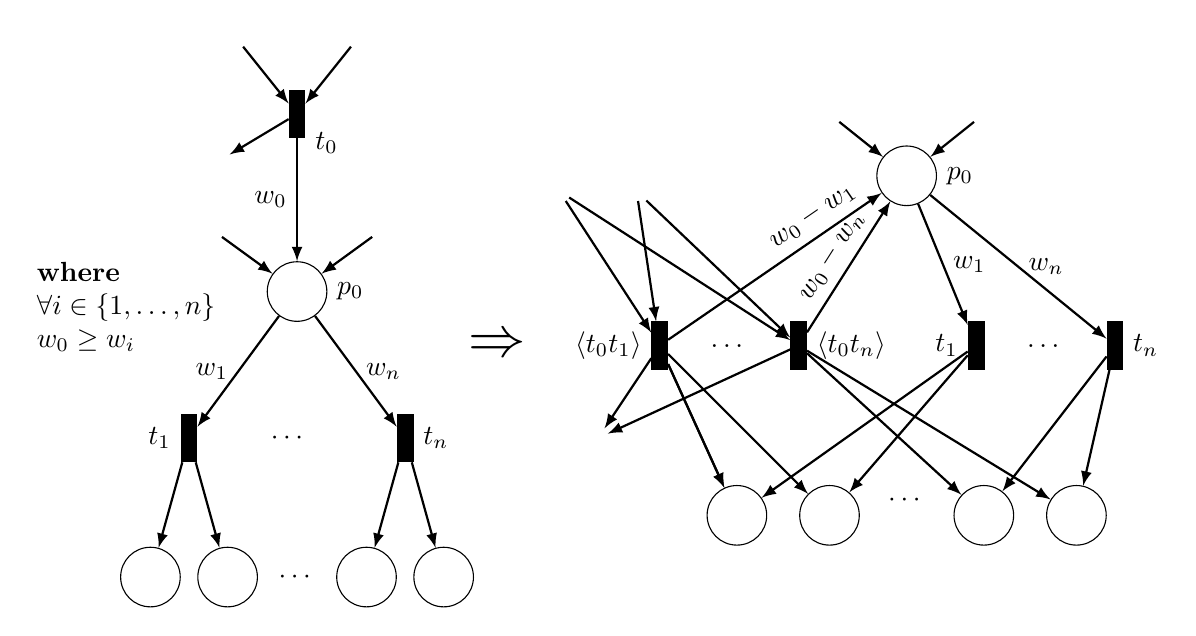
\begin{tikzpicture}[scale=0.98]
                % Left places
                \node[place,label=right:$p_0$] (rp) at (0.1,.7) {};
                \node[] (rph1) at (-.7,4) {};
                \node[] (rph2) at (.9,4) {};
                \node[] (rph1out) at (-.9,2.4) {};
                \node[place] (rpf1) at (-1.8,-3) {};
                \node[place] (rpf2) at (-0.8,-3) {};
                \node[place] (rpf3) at (1,-3) {};
                \node[place] (rpf4) at (2,-3) {};
                \node at (0.1,-3) {$\cdots$};

                % Left transitions
                \node[transition,minimum height=6mm,minimum width=2mm,fill=black,label=below right:$t_0$] (rh) at (0.1,3) {};
                \node[] (rh2) at (-1,1.5) {};
                \node[] (rh3) at (1.2,1.5) {};
                \node[transition,minimum height=6mm,minimum width=2mm,fill=black,label=left:$t_1$] (rf1) at (-1.3,-1.2) {};
                \node[transition,minimum height=6mm,minimum width=2mm,fill=black,label=right:$t_n$] (rf2) at (1.5,-1.2) {};
                \node at (0,-1.2) {$\cdots$};

                % Left arcs
                \draw[-latex,thick] (rph1) -- (rh);
                \draw[-latex,thick] (rph2) -- (rh);
                \draw[-latex,thick] (rh) edge node[left] {$w_0$} (rp);
                \draw[-latex,thick] (rh) -- (rph1out);
                \draw[-latex,thick] (rh2) -- (rp);
                \draw[-latex,thick] (rh3) -- (rp);
                \draw[-latex,thick] (rp) edge node[left] {$w_1$} (rf1);
                \draw[-latex,thick] (rp) edge node[right] {$w_n$} (rf2);
                \draw[-latex,thick] (rf1) -- (rpf1);
                \draw[-latex,thick] (rf1) -- (rpf2);
                \draw[-latex,thick] (rf2) -- (rpf3);
                \draw[-latex,thick] (rf2) -- (rpf4);

                % ================== Middle arrow ==================
                \node (arrow) at (2.7,0) {\huge$\Rightarrow$};
                % ==================================================

                % Right places
                \node[] (lph1) at (3.5,2) {};
                \node[] (lph2) at (4.5,2) {};
                \node[] (lhout) at (4,-1.2) {};
                \node[place,label=right:$p_0$] (lp) at (8,2.2) {};
                \node[place] (lpf1) at (5.8,-2.2) {};
                \node[place] (lpf2) at (7,-2.2) {};
                \node[place] (lpf3) at (9,-2.2) {};
                \node[place] (lpf4) at (10.2,-2.2) {};
                \node at (8,-2) {$\cdots$};

                % Right transitions
                \node (lh2) at (7,3) {};
                \node (lh3) at (9,3) {};
                \node[transition,minimum height=6mm,minimum width=2mm,fill=black,label=left:$\langle t_0t_1\rangle$] (lhf1f1) at (4.8,0) {};
                \node at (5.7,0) {$\dots$};
                \node[transition,minimum height=6mm,minimum width=2mm,fill=black,label=right:$\langle t_0t_n\rangle$] (lhf2f2) at (6.6,0) {};
                \node[transition,minimum height=6mm,minimum width=2mm,fill=black,label=left:$t_1$] (lf1) at (8.9,0) {};
                \node at (9.8,0) {$\dots$};
                \node[transition,minimum height=6mm,minimum width=2mm,fill=black,label=right:$t_n$] (lf2) at (10.7,0) {};

                % Right arcs above
                \draw[-latex,thick] (lhf1f1) edge[sloped, above right] node {$w_0-w_1$} (lp);
                \draw[-latex,thick] (lhf2f2) edge[sloped, above] node {$w_0-w_n$} (lp);
                \draw[-latex,thick] (lph1) -- (lhf1f1);
                \draw[-latex,thick] (lph1) -- (lhf2f2);
                \draw[-latex,thick] (lph2) -- (lhf1f1);
                \draw[-latex,thick] (lph2) -- (lhf2f2);
                \draw[-latex,thick] (lh2) -- (lp);
                \draw[-latex,thick] (lh3) -- (lp);
                \draw[-latex,thick] (lp) edge node[right] {$w_1$} (lf1);
                \draw[-latex,thick] (lp) edge node[right] {$w_n$} (lf2);

                % Right arcs below
                \draw[-latex,thick] (lhf1f1) -- (lhout);
                \draw[-latex,thick] (lhf2f2) -- (lhout);
                \draw[-latex,thick] (lhf1f1) -- (lpf1);
                \draw[-latex,thick] (lhf1f1) -- (lpf1);
                \draw[-latex,thick] (lhf1f1) -- (lpf2);
                \draw[-latex,thick] (lhf2f2) -- (lpf3);
                \draw[-latex,thick] (lhf2f2) -- (lpf4);
                \draw[-latex,thick] (lf1) -- (lpf1);
                \draw[-latex,thick] (lf1) -- (lpf2);
                \draw[-latex,thick] (lf2) -- (lpf3);
                \draw[-latex,thick] (lf2) -- (lpf4);

                % Right labels with background
                %\node[above=3pt of lhf1f1,outer sep=1pt,fill=white] {$h f_1\dots f_1$};
                %\node[above=3pt of lhf2f2,outer sep=1pt,fill=white] {$h f_2\dots f_2$};

                % Right lower weights
                \node[text width=7cm] at (.3,0.5) {\textbf{where }\\ $\forall i\in\{1,\dotsc,n\}$\\$w_0\geq w_i$};

            \end{tikzpicture}
        \end{adjustbox}
        \vspace{5mm}

        \begin{adjustbox}{center}
            \begin{tabular}{|p{68mm}|p{75mm}|} \hline
            Precondition & Update \\ \hline
            Fix place $p_0$ and transition $t_0$ s.t.:
            \begin{itemize}[leftmargin=10mm]
                \item[R1)] $t_0\in {}^\bullet p_0\land p_0^\bullet\neq\emptyset$
                \item[R2)] $^\bullet p_0 \cap p_0^\bullet = \emptyset$
                \item[R3)] $p_0 ^\circ = {}^\circ (p_0^\bullet) = ((p_0^\bullet)^\bullet)^\circ = \emptyset$
                \item[R4)] $(\{p_0\} \cup (p_0^\bullet)^\bullet) \cap places(\varphi) = \emptyset$
                \item[R5)] ${}^\bullet (p_0^\bullet)=\{p_0\}$
                \item[R6)] $\boxplus(t_0, p_0)\geq \boxminus(p_0,t)$ for all $t\in p_0^\bullet$
            \end{itemize} &

            \begin{itemize}[leftmargin=10mm]
                \item[UR1)]
                For each transition $t \in p_0^\bullet$ create a transition $\langle t_0 t\rangle$ with the following arcs:

                $\boxminus(\langle t_0 t\rangle)=\boxminus(t_0)$

                $\boxplus(\langle t_0 t\rangle)=\boxplus(t_0)+\boxplus(t)-\boxminus(t)$

                $I(\langle t_0 t\rangle)=I(t_0)$

                \item[UR2)] Remove $t_0$
            \end{itemize} \\ \hline
            \end{tabular}
        \end{adjustbox}
        \caption{Rule R: Atomic post-agglomerable producer}
        \label{fig:rule_r}
    \end{figure}

    \begin{theorem}
        Rule~R in Figure~\ref{fig:rule_r} is correct for LTL\textbackslash X.
    \end{theorem}

\end{document}

    \clearpage
    \section*{Rule S: Atomic free agglomeration (P/T)}\label{sec:rule_s}
A free agglomeration is a pre agglomeration, which does not require that the pre set of the preset of $p_0$ has a single consumer.
In turn, it is only correct for reachability with deadlocks.
The atomic free agglomeration is similar to the free agglomeration, but is able to agglomeration one consumer at a time.
See Figure~\ref{fig:rule_s} for its definition.
Rule~S also handles cases where the producer $h$ produces $k$ times more tokens than what the consumer $f_0$ consumes.
In this case, a transition $\langle h f_0^i\rangle$ is created for each $i\in [1, k]$.
Thus all relevant markings remain reachable.

\begin{figure}[h!]
    \centering
    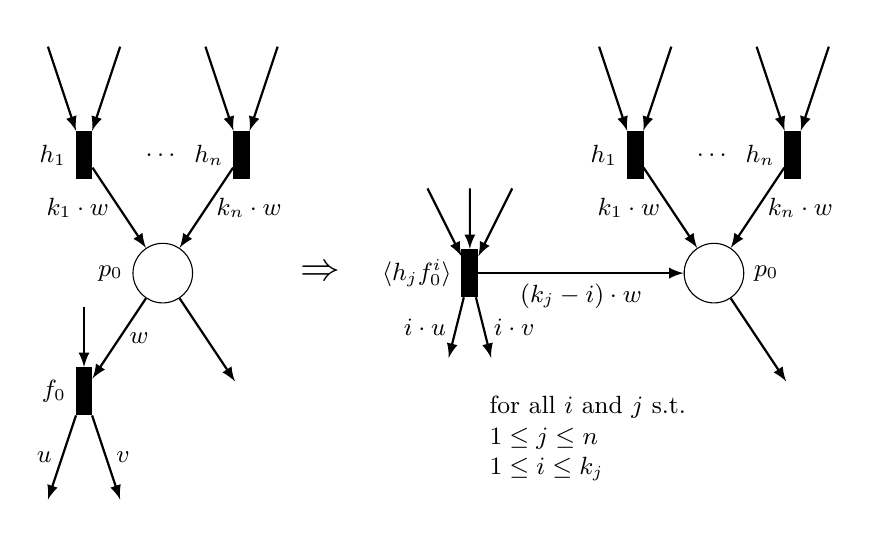
\begin{tikzpicture}
        \tikzstyle{every node}=[font=\small]
        %%% Before
        \begin{scope}[scale=0.5]
            \node[place,label=left:$p_0$] (p0) at (0,0) {};
            \node (h1pre1) at (-3,6) {};
            \node (h1pre2) at (-1,6) {};
            \node (hnpre1) at (1,6) {};
            \node (hnpre2) at (3,6) {};
            \node (f1pre) at (-2,-.6) {};
            \node (f1post1) at (-3,-6) {};
            \node (f1post2) at (-1,-6) {};
            \node (fmpre) at (3,-1) {};
            \node (fmpost1) at (1,-6) {};
            \node (fmpost2) at (3,-6) {};
            \node (fm) at (2,-3) {};

            \node[transition,minimum height=6mm,minimum width=2mm,fill=black,label=left:$h_1$] (h1) at (-2,3) {};
            \node (hdots) at (0,3) {$\dots$};
            \node[transition,minimum height=6mm,minimum width=2mm,fill=black,label=left:$h_n$] (hn) at (2,3) {};
            \node[transition,minimum height=6mm,minimum width=2mm,fill=black,label=left:$f_0$] (f1) at (-2,-3) {};
            %\node (fdots) at (-2,-5) {$\dots$};
            %\node[transition,minimum height=6mm,minimum width=2mm,fill=black,label=left:$f_m$] (fm) at (2,-3) {};

            \draw[-latex,thick] (h1pre1) edge (h1);
            \draw[-latex,thick] (h1pre2) edge (h1);
            \draw[-latex,thick] (hnpre1) edge (hn);
            \draw[-latex,thick] (hnpre2) edge (hn);
            \draw[-latex,thick] (h1) edge node[left] {$k_1 \cdot w$} (p0);
            \draw[-latex,thick] (hn) edge node[right] {$k_n \cdot w$} (p0);
            \draw[-latex,thick] (p0) edge node[right] {$w$} (f1);
            \draw[-latex,thick] (p0) edge node[right] {} (fm);
            \draw[-latex,thick] (f1pre) edge (f1);
            \draw[-latex,thick] (f1) edge node[left] {$u$} (f1post1);
            \draw[-latex,thick] (f1) edge node[right] {$v$} (f1post2);
            %\draw[-latex,thick] (fmpre) edge (fm);
            %\draw[-latex,thick] (fm) edge (fmpost1);
            %\draw[-latex,thick] (fm) edge (fmpost2);
        \end{scope}

        \node (arrow) at (2,0) {\Large $\Rightarrow$};

        %%% After
        \begin{scope}[shift={(3,0)},scale=0.6]
            \node (p11) at (2.5,2) {};
            \node (p12) at (1.5,2) {};
            \node (p13) at (0.5,2) {};
            \node (p14) at (1,-2) {};
            \node (p15) at (2,-2) {};

            \node[text width=2.5cm] (explain) at (4,-3.5) {for all $i$ and $j$ s.t. $1\leq j\leq n$\\$1 \leq i\leq k_j$};
            \node[transition,minimum height=6mm,minimum width=2mm,fill=black,label=left:$\langle h_j f_0^{i}\rangle$] (hnfmk) at (1.5,0) {};

            \draw[-latex,thick] (hnfmk) edge node[left] {$i \cdot u$} (p14);
            \draw[-latex,thick] (hnfmk) edge node[right] {$i \cdot v$} (p15);
            \draw[-latex,thick] (p11) edge (hnfmk);
            \draw[-latex,thick] (p12) edge (hnfmk);
            \draw[-latex,thick] (p13) edge (hnfmk);

        \end{scope}
        \begin{scope}[shift={(7,0)}, scale=0.5]
            \node[place,label=right:$p_0$] (p0) at (0,0) {};
            \node (h1pre1) at (-3,6) {};
            \node (h1pre2) at (-1,6) {};
            \node (hnpre1) at (1,6) {};
            \node (hnpre2) at (3,6) {};
            %\node (f1pre) at (-3,-1) {};
            %\node (f1post1) at (-3,-6) {};
            %\node (f1post2) at (-1,-6) {};
            \node (fmpre) at (3,-1) {};
            \node (fmpost1) at (1,-6) {};
            \node (fmpost2) at (3,-6) {};
            \node (fm) at (2,-3) {};

            \node[transition,minimum height=6mm,minimum width=2mm,fill=black,label=left:$h_1$] (h1) at (-2,3) {};
            \node (hdots) at (0,3) {$\dots$};
            \node[transition,minimum height=6mm,minimum width=2mm,fill=black,label=left:$h_n$] (hn) at (2,3) {};
            %\node[transition,minimum height=6mm,minimum width=2mm,fill=black,label=left:$f_0$] (f1) at (-2,-3) {};
            %\node (fdots) at (-2,-5) {$\dots$};
            %\node[transition,minimum height=6mm,minimum width=2mm,fill=black,label=left:$f_m$] (fm) at (2,-3) {};

            \draw[-latex,thick] (h1pre1) edge (h1);
            \draw[-latex,thick] (h1pre2) edge (h1);
            \draw[-latex,thick] (hnpre1) edge (hn);
            \draw[-latex,thick] (hnpre2) edge (hn);
            \draw[-latex,thick] (h1) edge node[left] {$k_1\cdot w$} (p0);
            \draw[-latex,thick] (hn) edge node[right] {$k_n\cdot w$} (p0);
            %\draw[-latex,thick] (p0) edge node[left] {$W$} (f1);
            \draw[-latex,thick] (p0) edge node[right] {} (fm);
            \draw[-latex,thick] (hnfmk) edge node[below] {$(k_j-i)\cdot w$} (p0);
            %\draw[-latex,thick] (f1pre) edge (f1);
            %\draw[-latex,thick] (f1) edge node[left] {} (f1post1);
            %\draw[-latex,thick] (f1) edge node[right] {} (f1post2);
            %\draw[-latex,thick] (fmpre) edge (fm);
            %\draw[-latex,thick] (fm) edge (fmpost1);
            %\draw[-latex,thick] (fm) edge (fmpost2);
        \end{scope}
    \end{tikzpicture}
    \vspace{5mm}

    \begin{adjustbox}{center}
        \begin{tabular}{|p{75mm}|p{75mm}|} \hline
        Precondition & Update \\ \hline
        Fix place $p_0$ and transition $f_0$ s.t.:
        \begin{itemize}[leftmargin=10mm]
            \item[S1)] $\{p_0\} \cap places(\varphi) = \emptyset$
            \item[S2)] $(f_0 \cup {}^\bullet p_0) \cap transitions(\varphi) = \emptyset$
            \item[S3)] $M_0(p_0) < \boxminus(p_0,f_0)$
            \item[S4)] $^\bullet p_0 \cap p_0^\bullet = \emptyset$
            \item[S5)] $f_0 \in p_0^\bullet$
        \end{itemize}
        \hspace{2mm}
        \noindent and for all $h\in{}^\bullet p_0$ there exists a $k\in\N$ s.t.:
        \begin{itemize}[leftmargin=10mm]
            \item[S6)] $h^\bullet=\{p_0\}$
            \item[S7)] ${}^\bullet h \cap places(\varphi) = \emptyset$
            \item[S8)] $p_0^\circ = {}^\circ h = ({}^\bullet h)^\circ = \emptyset$
            \item[S9)] $\boxplus(h, p_0) = k\cdot\boxminus(p_0,f_0)$
            \item[S10)] $k > 1 \implies (f_0^\bullet)^\circ = \emptyset$
            \item[S11)] $k > 1 \implies{}^\bullet f_0 = \{p_0\}$
        \end{itemize}
        \hspace{2mm}

        &
        Create transition $\langle hf_0^i\rangle$ for all $i \in [1, k]$, for $k = \boxplus(h,p_0)/\boxminus(p_0,f_0)$, for all $h\in{}^\bullet p_0$.
        For each such transition:
        \begin{itemize}[leftmargin=12mm]
            \item[US1)] $\boxplus(\langle hf_0^i\rangle,p_0)=\boxplus(h,p_0) - i\cdot\boxminus(p,f_0)$
        \end{itemize}
        \hspace{2mm}
        \noindent and for all $p\in P\setminus\{p_0\}$:
        \begin{itemize}[leftmargin=12mm]
            \item[US2)] $\boxminus(p,\langle hf_0^i\rangle)=\boxminus(p,h)\uplus\boxminus(p,f_0)$
            \item[US3)] $\boxplus(\langle hf_0^i\rangle,p)=i\cdot\boxplus(f_0,p)$
            \item[US4)] $I(p,\langle hf_0^i\rangle) = I(p,f_0)$
        \end{itemize}
        \hspace{2mm}
        \noindent and
        \begin{itemize}[leftmargin=12mm]
            \item[US5)] Remove $f_0$
            \item[US6)] If $p_0^\bullet = \emptyset$, remove $p_0$ and all transitions in ${}^\bullet p_0\setminus transitions(\varphi)$
        \end{itemize} \\ \hline
        \end{tabular}
    \end{adjustbox}
    \caption{Rule S: Atomic free agglomeration}
    \label{fig:rule_s}
\end{figure}

\begin{theorem}
    Rule~S shown in Figure~\ref{fig:rule_s} is correct for deadlock-insensitive reachability properties.
\end{theorem}

    \clearpage
    \section*{Rule T: Pre agglomearation}\label{sec:rule_t}

Rule~T in Figure~\ref{fig:rule_t} is a pre agglomeration.
In a pre agglomeration $h\in{}^\bullet p_0$ is invisible to the query and once enabled, it stays enabled.
Hence, it can be delayed until an $f\in p_0^\bullet$ needs it.
Thus Rule~T creates a transition $\langle h f\rangle$ for every pair $h\in{}^\bullet p_0$ and $f\in p_0^\bullet$.

\begin{theorem}
    Rule~T described in Figure~\ref{fig:rule_t} is correct for LTL\textbackslash X.
\end{theorem}

\begin{figure}[h!]
    \centering
    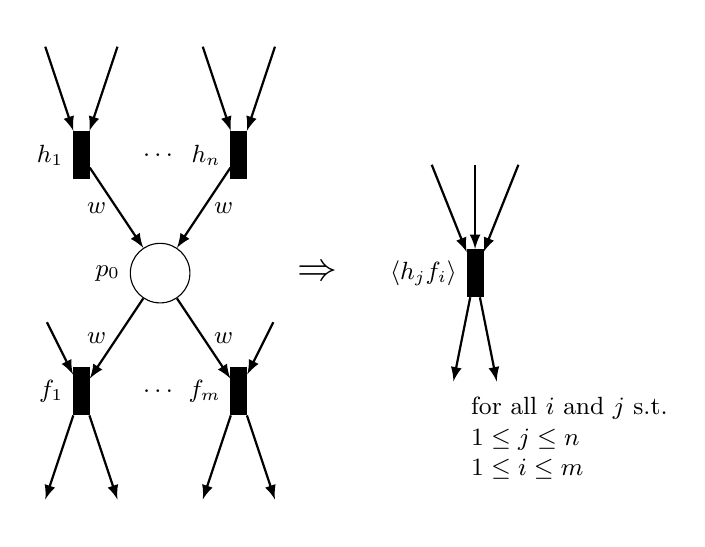
\begin{tikzpicture}
        \tikzstyle{every node}=[font=\small]
        %%% Before
        \begin{scope}[scale=0.5]
            \node[place,label=left:$p_0$] (p0) at (0,0) {};
            \node (h1pre1) at (-3,6) {};
            \node (h1pre2) at (-1,6) {};
            \node (hnpre1) at (1,6) {};
            \node (hnpre2) at (3,6) {};
            \node (f1pre) at (-3,-1) {};
            \node (f1post1) at (-3,-6) {};
            \node (f1post2) at (-1,-6) {};
            \node (fmpre) at (3,-1) {};
            \node (fmpost1) at (1,-6) {};
            \node (fmpost2) at (3,-6) {};
            \node (fm) at (2,-3) {};

            \node[transition,minimum height=6mm,minimum width=2mm,fill=black,label=left:$h_1$] (h1) at (-2,3) {};
            \node (hdots) at (0,3) {$\dots$};
            \node (fdots) at (0,-3) {$\dots$};
            \node[transition,minimum height=6mm,minimum width=2mm,fill=black,label=left:$h_n$] (hn) at (2,3) {};
            \node[transition,minimum height=6mm,minimum width=2mm,fill=black,label=left:$f_1$] (f1) at (-2,-3) {};
            \node[transition,minimum height=6mm,minimum width=2mm,fill=black,label=left:$f_m$] (fm) at (2,-3) {};
            %\node (fdots) at (-2,-5) {$\dots$};
            %\node[transition,minimum height=6mm,minimum width=2mm,fill=black,label=left:$f_m$] (fm) at (2,-3) {};

            \draw[-latex,thick] (h1pre1) edge (h1);
            \draw[-latex,thick] (h1pre2) edge (h1);
            \draw[-latex,thick] (hnpre1) edge (hn);
            \draw[-latex,thick] (hnpre2) edge (hn);
            \draw[-latex,thick] (h1) edge node[left] {$w$} (p0);
            \draw[-latex,thick] (hn) edge node[right] {$w$} (p0);
            \draw[-latex,thick] (p0) edge node[left] {$w$} (f1);
            \draw[-latex,thick] (p0) edge node[right] {$w$} (fm);
            \draw[-latex,thick] (f1pre) edge (f1);
            \draw[-latex,thick] (f1) edge(f1post1);
            \draw[-latex,thick] (f1) edge (f1post2);
            \draw[-latex,thick] (fmpre) edge (fm);
            \draw[-latex,thick] (fm) edge (fmpost1);
            \draw[-latex,thick] (fm) edge (fmpost2);
        \end{scope}

        \node (arrow) at (2,0) {\Large $\Rightarrow$};

        %%% After
        \begin{scope}[shift={(4,0)},scale=0.6]
            \node (p1) at (-1,2.5) {};
            \node (p2) at (0,2.5) {};
            \node (p9) at (1,2.5) {};
    %            \node (p3) at (1,2.5) {};
    %            \node (p4) at (2,2.5) {};
    %            \node (p10) at (3,2.5) {};
            \node (p5) at (-0.5,-2.5) {};
            \node (p6) at (0.5,-2.5) {};
    %            \node (p7) at (1.5,-2.5) {};
    %            \node (p8) at (2.5,-2.5) {};

            \node[transition,minimum height=6mm,minimum width=2mm,fill=black,label=left:$\langle h_j f_i \rangle$] (hjfi) at (0,0) {};
            \node[text width=2.5cm] (explain) at (2,-3.5) {for all $i$ and $j$ s.t. $1\leq j\leq n$\\$1 \leq i\leq m$};

            \draw[-latex,thick] (p1) edge (hjfi);
            \draw[-latex,thick] (p2) edge (hjfi);
            \draw[-latex,thick] (p9) edge (hjfi);
            % \draw[-latex,thick] (p3) edge (hnfm);
            % \draw[-latex,thick] (p4) edge (hnfm);
            % \draw[-latex,thick] (p10) edge (hnfm);
            \draw[-latex,thick] (hjfi) edge (p5);
            \draw[-latex,thick] (hjfi) edge (p6);
            % \draw[-latex,thick] (hnfm) edge node[left] {} (p7);
        \end{scope}
%        \begin{scope}[shift={(7,0)}, scale=0.5]
%%            \node[place,label=right:$p_0$] (p0) at (0,0) {};
%%            \node (h1pre1) at (-3,6) {};
%%            \node (h1pre2) at (-1,6) {};
%%            \node (hnpre1) at (1,6) {};
%%            \node (hnpre2) at (3,6) {};
%%            %\node (f1pre) at (-3,-1) {};
%%            %\node (f1post1) at (-3,-6) {};
%%            %\node (f1post2) at (-1,-6) {};
%%            \node (fmpre) at (3,-1) {};
%%            \node (fmpost1) at (1,-6) {};
%%            \node (fmpost2) at (3,-6) {};
%%            \node (fm) at (2,-3) {};
%
%%            \node[transition,minimum height=6mm,minimum width=2mm,fill=black,label=left:$h_1$] (h1) at (-2,3) {};
%%            \node (hdots) at (0,3) {$\dots$};
%%            \node[transition,minimum height=6mm,minimum width=2mm,fill=black,label=left:$h_n$] (hn) at (2,3) {};
%            %\node[transition,minimum height=6mm,minimum width=2mm,fill=black,label=left:$f_0$] (f1) at (-2,-3) {};
%            %\node (fdots) at (-2,-5) {$\dots$};
%            %\node[transition,minimum height=6mm,minimum width=2mm,fill=black,label=left:$f_m$] (fm) at (2,-3) {};
%
%            \draw[-latex,thick] (h1pre1) edge (h1);
%            \draw[-latex,thick] (h1pre2) edge (h1);
%            \draw[-latex,thick] (hnpre1) edge (hn);
%            \draw[-latex,thick] (hnpre2) edge (hn);
%            \draw[-latex,thick] (h1) edge node[left] {$w'x$} (p0);
%            \draw[-latex,thick] (hn) edge node[right] {$w'x$} (p0);
%            %\draw[-latex,thick] (p0) edge node[left] {$W$} (f1);
%            \draw[-latex,thick] (p0) edge node[right] {} (fm);
%            \draw[-latex,thick] (hjfi) edge node[below] {$((k_j-i)  \cdot  w)'x$} (p0);
%            %\draw[-latex,thick] (f1pre) edge (f1);
%            %\draw[-latex,thick] (f1) edge node[left] {} (f1post1);
%            %\draw[-latex,thick] (f1) edge node[right] {} (f1post2);
%            %\draw[-latex,thick] (fmpre) edge (fm);
%            %\draw[-latex,thick] (fm) edge (fmpost1);
%            %\draw[-latex,thick] (fm) edge (fmpost2);
%        \end{scope}
    \end{tikzpicture}
    \vspace{5mm}
    \begin{adjustbox}{center}
        \begin{tabular}{|p{75mm}|p{75mm}|} \hline
        Precondition & Update \\ \hline
        Fix place $p_0$ s.t.:
        \begin{itemize}[leftmargin=10mm]
            \item[T1)] $(\{p_0\} \cap places(\varphi) = \emptyset$
            \item[T2)] $(p_0^\bullet \cup {}^\bullet p_0) \cap transitions(\varphi) = \emptyset$
        \end{itemize}
        \noindent for all $h\in{}^\bullet p_0$ and $f \in p_0^\bullet$:
        \begin{itemize}[leftmargin=10mm]
            \item[T3)] $M_0(p_0) < \boxminus(p_0,f)$
            \item[T4)] $^\bullet p_0 \cap p_0^\bullet = \emptyset$
            \item[T5)] $({}^\bullet h)^\bullet = \{h\}$
            \item[T6)] $h^\bullet=\{p_0\}$
            \item[T7)] ${}^\bullet h \cap places(\varphi) = \emptyset$
            \item[T8)] $p_0^\circ = {}^\circ h = ({}^\bullet h)^\circ = \emptyset$
            \item[T9)] $\boxplus(h, p_0) = \boxminus(p_0,f)$
        \end{itemize}

        % additionally, for any $k$ that satisfied S8):
        % \begin{itemize}[leftmargin=10mm]
        %     \item[S9)] $k > 1 \implies (f_0^\bullet)^\circ = \emptyset$
        %     \item[S10)] $k > 1 \implies{}^\bullet f_0 = \{p_0\}$
        % \end{itemize}

        &
        Create transition $\langle hf\rangle$ for all $h\in{}^\bullet p_0$ and $f\in p_0^\bullet$ s.t.\ for all $p\in P\setminus\{p_0\}$:
        \begin{itemize}[leftmargin=12mm]
            \item[UT1)] $\boxminus(p,\langle hf\rangle)=\boxminus(p,h)+\boxminus(p,f)$
            \item[UT2)] $\boxplus(\langle hf\rangle,p)=\boxplus(f,p)$
            \item[UT3)] $I(p,\langle hf\rangle) = I(p,f)$
        \end{itemize}
        \noindent and
        \begin{itemize}[leftmargin=12mm]
            \item[UT4)] Remove ${}^\bullet p_0$, $p_0^\bullet $ and $p_0$

        \end{itemize} \\ \hline
        \end{tabular}
    \end{adjustbox}
    \caption{Rule T: Pre agglomeration}
    \label{fig:rule_t}
\end{figure}
    % Colored reductions
    \clearpage
    \section*{Rule C: Parallel place removal (CPN)}\label{sec:rule_c_cpn}
When two places are symmetrically parallel to each other and one may accumulate tokens, Rule~C will remove it.
See Figure~\ref{fig:rule_c_cpn}.
By convention $\min\emptyset=-\infty$ and $\max\emptyset=\infty$.
The fraction $d$ describes how fast tokens can be consumed from $p_2$ compared to $p_1$,
while $f$ describes how slow tokens can be fed to $p_2$ compared to $p_1$.
If $d\leq f$ then $p_2$ is always fed faster than it is emptied compared to $p_1$,
which means $p_2$ can be removed, since it will always be $p_1$ which is missing tokens and disables their consumers.

\begin{figure}[h!]
    \centering
    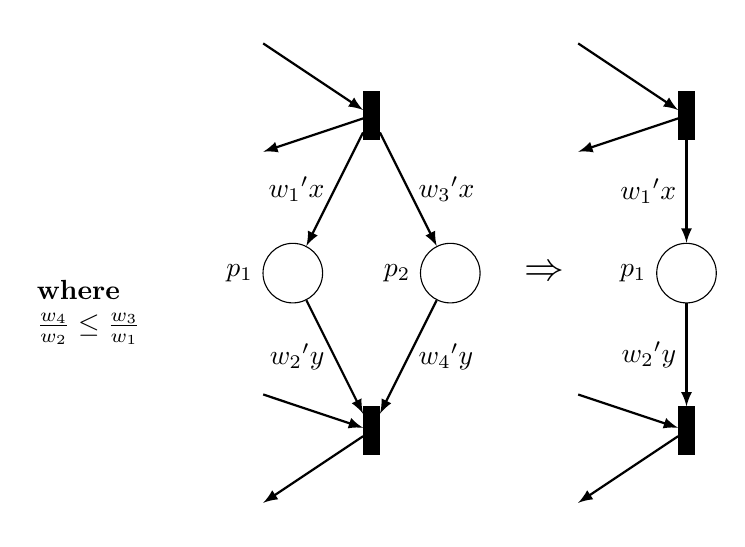
\begin{tikzpicture}
        %%% Before
        \begin{scope}
            % Places
            \node[place, label=left:$p_1$] (place1) at (-1,0) {};
            \node[place, label=left:$p_2$] (place2) at (1,0) {};

            % Transitions
            \node[transition,minimum height=6mm,minimum width=2mm,fill=black] (lTrans1) at (0,2) {};
            \node[transition,minimum height=6mm,minimum width=2mm,fill=black] (lTrans2) at (0,-2) {};

            % Invisible nodes
            \node (negIn1) at (-1.5,3) {};
            \node (negOut1) at (-1.5,1.5) {};
            \node (remIn1) at (-1.5,-1.5) {};
            \node (remOut1) at (-1.5,-3) {};

            % Arcs between transitions and places
            \draw[-latex,thick] (lTrans1) to node[left] {$w_1{}'x$} (place1);
            \draw[-latex,thick] (lTrans1) to node[right] {$w_3{}'x$} (place2);
            \draw[-latex,thick] (place1) to node[left] {$w_2{}'y$} (lTrans2);
            \draw[-latex,thick] (place2) to node[right] {$w_4{}'y$} (lTrans2);

            % Arcs to/from invisible nodes
            \draw[-latex,thick] (negIn1) -- node[above] {} (lTrans1);
            \draw[-latex,thick]  (remIn1) -- node[below] {} (lTrans2);
            \draw[-latex,thick]  (lTrans2) -- node[below] {} (remOut1);
            \draw[-latex,thick]  (lTrans1) -- node[above] {} (negOut1);
        \end{scope}

        \node (arrow) at (2.2,0) {\Large$\Rightarrow$};
        \node[text width=3.5cm] at (-2.5,-0.5) {\textbf{where }\\$\frac{w_4}{w_2}\leq\frac{w_3}{w_1}$};

        \begin{scope}
            % Places
            \node[place, label=left:$p_1$] (rplace1) at (4,0) {};

            % Transitions
            \node[transition,minimum height=6mm,minimum width=2mm,fill=black] (rTrans1) at (4,2) {};
            \node[transition,minimum height=6mm,minimum width=2mm,fill=black] (rTrans2) at (4,-2) {};

            % Arcs between transitions and places
            \draw[-latex,thick] (rTrans1) to node[left] {$w_1{}'x$} (rplace1);
            \draw[-latex,thick] (rplace1) to node[left] {$w_2{}'y$} (rTrans2);

            % Invisible nodes
            \node (rnegIn1) at (2.5,3) {};
            \node (rnegOut1) at (2.5,1.5) {};
            \node (rremIn1) at (2.5,-1.5) {};
            \node (rremOut1) at (2.5,-3) {};

            % Arcs to/from invisible nodes
            \draw[-latex,thick] (rnegIn1) -- node[above] {} (rTrans1);
            \draw[-latex,thick]  (rremIn1) -- node[below] {} (rTrans2);
            \draw[-latex,thick]  (rTrans2) -- node[below] {} (rremOut1);
            \draw[-latex,thick]  (rTrans1) -- node[above] {} (rnegOut1);
        \end{scope}
    \end{tikzpicture}
    \vspace{5mm}
    \begin{adjustbox}{center}
        \begin{tabular}{|p{75mm}|p{45mm}|} \hline
        Precondition & Update \\ \hline
        Fix places $p_1$ and $p_2$ s.t.:
        \begin{itemize}[leftmargin=10mm]
            \item[C1)] $\mathcal X(p_1)=\mathcal X(p_2)$
            \item[C2)] $p_2\notin places(\varphi)$
            \item[C3)] $p_2^\circ=\emptyset$
            \item[C4)] $p_1^\bullet\neq\emptyset$
            \item[C5)] For all $t\in T$:

            $\textbf{Supp}(\boxminus(p_1, t))=\textbf{Supp}(\boxminus(p_2, t))\land$

            $\textbf{Supp}(\boxplus(t, p_1))=\textbf{Supp}(\boxplus(t, p_2))$

            \item[C6)] $\textbf{Supp}(M_0(p_1))=\textbf{Supp}(M_0(p_2))\land$

            $M_0(p_1)\cdot d \subseteq M_0(p_2)$
            \item[C7)] $d\leq f$
        \end{itemize}
        where
        \[
            d = \max_{t\in p_1^\bullet,V\in \boxminus(p_1, t)}\frac{\boxminus(p_2, t)(V)}{\boxminus(p_1, t)(V)}
        \]
        \[
            f = \min_{t\in{}^\bullet p_1,V\in \boxplus(t, p_1)}\frac{\boxplus(t, p_2)(V)}{\boxplus(t, p_1)(V)}
        \]
        &
        \begin{itemize}[leftmargin=10mm]
            \item[UC1)] remove $p_2$
        \end{itemize} \\ \hline
        \end{tabular}
    \end{adjustbox}
    \caption{Rule C: Parallel places (CPN)}
    \label{fig:rule_c_cpn}
\end{figure}

\begin{theorem}
    Rule~C shown in Figure~\ref{fig:rule_c_cpn} are correct for CTL* properties.
\end{theorem}

    \clearpage
    \section*{Rule D: Parallel transitions}\label{sec:rule_d_cpn}
Rule~D handles parallel transitions where the effect of firing one of them is equivalent to firing the other exactly $k$ times.
In such a case, we remove the transition with higher arc-weights.
The definition of Rule~D can be seen in Figure~\ref{fig:rule_d_cpn}.
In precondition D2 states that the valid bindings of the guard $G(t_1)$ must be a subset of the valid bindings of $G(t_2)$,
i.e.\ $\vec B(t_1)\subseteq\vec B(t_2)$.
This can be expensive to check depending on the complexity of the guards and the number of variables in the guard.
A cheap overapproximation is to check whether $G(t_1)=G(t_2)$ or $G(t_2)=\top$ instead.

\begin{figure}[h!]
    \centering
    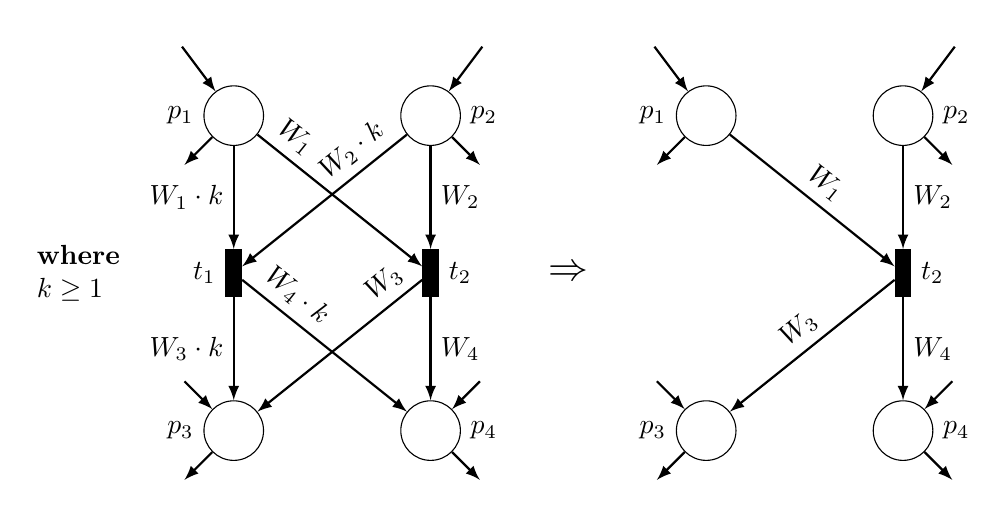
\begin{tikzpicture}
        \begin{scope}
            % left side Places
            \node[place, label=left:$p_1$] (place1) at (-1.25,2) {};
            \node[place, label=right:$p_2$] (place2) at (1.25,2) {};
            \node[place, label=left:$p_3$] (place3) at (-1.25,-2) {};
            \node[place, label=right:$p_4$] (place4) at (1.25,-2) {};

            % Left side transitions
            \node[transition,minimum height=6mm,minimum width=2mm,fill=black, label=right:$t_2$] (lTrans2) at (1.25,0) {};
            \node[transition,minimum height=6mm,minimum width=2mm,fill=black, label=left:$t_1$] (lTrans1) at (-1.25,0) {};

            % Left side invisible nodes
            \node (place1in) at (-2,3) {};
            \node (place1out) at (-2,1.25) {};
            \node (place2in) at (2,3) {};
            \node (place2out) at (2,1.25) {};

            \node (place3in) at (-2,-1.25) {};
            \node (place3out) at (-2,-2.75) {};
            \node (place4in) at (2,-1.25) {};
            \node (place4out) at (2,-2.75) {};

            % Left side arcs between transitions and places
            \draw[-latex,thick] (place1) to node[left] {$W_1 \cdot k$} (lTrans1);
            \draw[-latex,thick] (place1) to node[sloped, above, pos=0.15] {$W_1$} (lTrans2);
            \draw[-latex,thick] (place2) to node[sloped, above, pos=0.25] {$W_2 \cdot k$} (lTrans1);
            \draw[-latex,thick] (place2) to node[right] {$W_2$} (lTrans2);

            \draw[-latex,thick] (lTrans1) to node[left] {$W_3 \cdot k$} (place3);
            \draw[-latex,thick] (lTrans1) to node[sloped, above, pos=0.25] {$W_4 \cdot k$} (place4);
            \draw[-latex,thick] (lTrans2) to node[sloped, above, pos=0.15] {$W_3$} (place3);
            \draw[-latex,thick] (lTrans2) to node[right] {$W_4$} (place4);


            % Left side arcs to/from invisible nodes
            \draw[-latex,thick] (place1in) -- node[above] {} (place1);
            \draw[-latex,thick]  (place1) -- node[below] {} (place1out);
            \draw[-latex,thick]  (place2in) -- node[below] {} (place2);
            \draw[-latex,thick]  (place2) -- node[above] {} (place2out);

            \draw[-latex,thick] (place3in) -- node[above] {} (place3);
            \draw[-latex,thick]  (place3) -- node[below] {} (place3out);
            \draw[-latex,thick]  (place4in) -- node[below] {} (place4);
            \draw[-latex,thick]  (place4) -- node[above] {} (place4out);
        \end{scope}
        % ================== Middle arrow ==================
        \node (arrow) at (3,0) {\Large$\Rightarrow$};
        \node[text width=3.5cm] at (-2,0) {\textbf{where }\\$k\geq 1$};
        % ==================================================
        \begin{scope}[shift={(6, 0)}]


        % left side Places
        \node[place, label=left:$p_1$] (place1) at (-1.25,2) {};
        \node[place, label=right:$p_2$] (place2) at (1.25,2) {};
        \node[place, label=left:$p_3$] (place3) at (-1.25,-2) {};
        \node[place, label=right:$p_4$] (place4) at (1.25,-2) {};

        % Left side transitions
        \node[transition,minimum height=6mm,minimum width=2mm,fill=black, label=right:$t_2$] (lTrans2) at (1.25,0) {};

        % Left side invisible nodes
        \node (place1in) at (-2,3) {};
        \node (place1out) at (-2,1.25) {};
        \node (place2in) at (2,3) {};
        \node (place2out) at (2,1.25) {};

        \node (place3in) at (-2,-1.25) {};
        \node (place3out) at (-2,-2.75) {};
        \node (place4in) at (2,-1.25) {};
        \node (place4out) at (2,-2.75) {};

        % Left side arcs between transitions and places
        \draw[-latex,thick] (place1) to node[sloped, above, pos=0.5] {$W_1$} (lTrans2);
        \draw[-latex,thick] (place2) to node[right] {$W_2$} (lTrans2);

        \draw[-latex,thick] (lTrans2) to node[sloped, above, pos=0.5] {$W_3$} (place3);
        \draw[-latex,thick] (lTrans2) to node[right] {$W_4$} (place4);


        % Left side arcs to/from invisible nodes
        \draw[-latex,thick] (place1in) -- node[above] {} (place1);
        \draw[-latex,thick]  (place1) -- node[below] {} (place1out);
        \draw[-latex,thick]  (place2in) -- node[below] {} (place2);
        \draw[-latex,thick]  (place2) -- node[above] {} (place2out);

        \draw[-latex,thick] (place3in) -- node[above] {} (place3);
        \draw[-latex,thick]  (place3) -- node[below] {} (place3out);
        \draw[-latex,thick]  (place4in) -- node[below] {} (place4);
        \draw[-latex,thick]  (place4) -- node[above] {} (place4out);
        \end{scope}

    \end{tikzpicture}
    \vspace{5mm}
    \begin{adjustbox}{center}
        \begin{tabular}{|p{75mm}|p{45mm}|} \hline
        Precondition & Update \\ \hline
        Fix transitions $t_1$ and $t_2$ and $k\in\N$ s.t.:
        \begin{itemize}[leftmargin=10mm]
            \item[D1)] $t_1\notin transitions(\varphi)$
            \item[D2)] $\vec B(t_1)\subseteq\vec B(t_2)$
            \item[D3)] $\varphi\in\text{CTL}\lor X\in\varphi\implies k=1$
            \item[D4)] For all $p\in P$:
            \begin{itemize}
                %\item[] $\textbf{Supp}(\boxplus(t,p_1)) = \textbf{Supp}(\boxplus(t,p_2))$
                \item[] $\boxminus(p, t_1) = \boxminus(p, t_2) \cdot k $
                \item[] $\boxplus(t_1, p) = \boxplus(t_2, p) \cdot k $
            \end{itemize}
            \item[D5)] ${}^\circ t_2\cap t_2^\bullet=\emptyset$
            \item[D6)] $\forall p \in P.I(p, t_1) \leq I(p, t_2)$
            \item[D7)] $\varphi\notin Reach\Rightarrow ({}^\bullet t_1\cup t_1^\bullet) \cap (places(\varphi)\cup{}^\bullet transitions(\varphi))=\emptyset$
        \end{itemize}
        &
        \begin{itemize}[leftmargin=12mm]
            \item[UD1)] remove $t_1$
        \end{itemize} \\ \hline
        \end{tabular}
    \end{adjustbox}
    \caption{Rule D: Parallel transitions}
    \label{fig:rule_d_cpn}
\end{figure}

\begin{theorem}
    Rule~D described in Figure~\ref{fig:rule_d_cpn} is correct for LTL\textbackslash X.
\end{theorem}

\begin{theorem}
    Rule~D described in Figure~\ref{fig:rule_d_cpn} is correct for CTL* if $k=1$.
\end{theorem}
    \clearpage
    \section*{Rule E: Dead transition removal (CPN)}\label{sec:rule_e_cpn}

Rule~E in Figure~\ref{fig:rule_e_cpn} removes transitions that are never enabled.
If too many bindings exists to check E1, then checking the cardinalities is a valid overapproximation.

Precondition E3 can be ignored $\varphi$ if all instances of $en(t_0)$ are replaced with $\neg\top$ instead in the update.

\begin{figure}[h!]
    \centering
    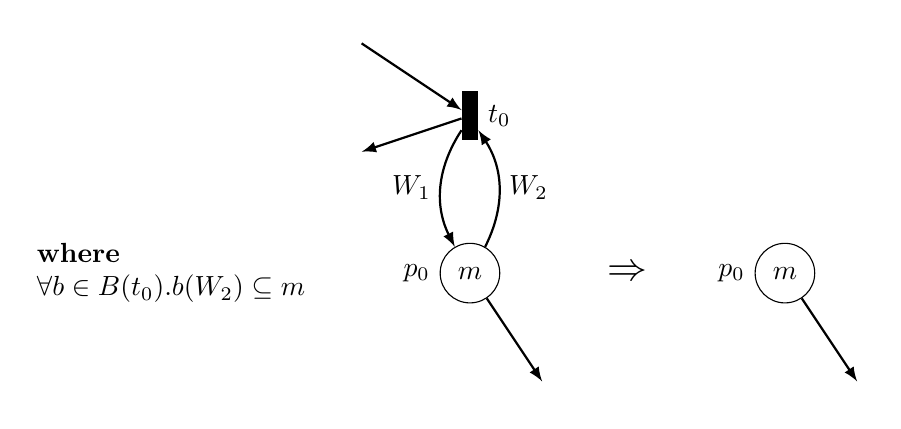
\begin{tikzpicture}
        % left side Places
        \node[place, label=left:$p_0$] (place1) at (0,0) {$m$};

        % Left side transitions
        \node[transition,minimum height=6mm,minimum width=2mm,fill=black,label=right:$t_0$] (lTrans1) at (0,2) {};

        % Left side invisible nodes
        \node (negIn1) at (-1.5,3) {};
        \node (negOut1) at (-1.5,1.5) {};
        \node (remIn1) at (-1.5,-1.5) {};
        \node (negOut2) at (1,-1.5) {};

        % Left side arcs between transitions and places
        \draw[-latex,thick] (lTrans1) edge [bend right] node [left] {$W_1$} (place1);
        \draw[-latex,thick] (place1) edge [bend right] node [right] {$W_2$} (lTrans1);

        % Left side arcs to/from invisible nodes
        \draw[-latex,thick] (negIn1) -- node[above] {} (lTrans1);
        \draw[-latex,thick]  (lTrans1) -- node[above] {} (negOut1);
        \draw[-latex,thick]  (place1) -- node[above] {} (negOut2);

        % ================== Middle arrow ==================
        \node (arrow) at (2,0) {\Large$\Rightarrow$};
        \node[text width=4cm] at (-3.5,0) {\textbf{where }\\$\forall b\in B(t_0).b(W_2)\subseteq m$};
        % ==================================================

        % right side transitions
        \node[place, label=left:$p_0$] (rplace1) at (4,0) {$m$};

        % right side invisible nodes
        \node (rnegIn1) at (2.5,3) {};
        \node (rnegOut1) at (2.5,1.5) {};
        \node (rremIn1) at (2.5,-1.5) {};
        \node (rremOut1) at (5,-1.5) {};

        % right side arcs to/from invisible nodes
        %\draw[-latex,thick] (rremIn1) -- node[above] {} (rplace1);
        \draw[-latex,thick] (rplace1) -- node[above] {} (rremOut1);

    \end{tikzpicture}
    \vspace{5mm}
    \begin{adjustbox}{center}
        \begin{tabular}{|p{65mm}|p{45mm}|}
            \hline
            Precondition & Update \\ \hline
            Fix place $p_0$ and transition $t_0$ s.t.:
            \begin{itemize}[leftmargin=10mm]
                \item[E1)] $\forall b\in B(t) . b(\boxminus(p_0,t_0))\not\subseteq M_0(p_0)$
                \item[E2)] $\forall t \in {}^\bullet p_0: \boxplus(t, p_0) \subseteq \boxminus(p_0,t)$ or $\forall b\in B(t) . b(\boxminus(p_0,t))\not\subseteq M_0(p_0)$
                \item[E3)] $t_0\notin transitions(\varphi)$
            \end{itemize}
            &
            \begin{itemize}[leftmargin=10mm]
                \item[UE1)] If $p_0 \not \in places(\varphi)$ and $p_0^\bullet = \{t_0\}$, remove $p_0$
                \item[UE2)] Remove $t_0$
            \end{itemize} \\ \hline
        \end{tabular}
    \end{adjustbox}
    \caption{Rule E: Dead transitions}
    \label{fig:rule_e_cpn}
\end{figure}

\begin{theorem}
    Rule~E in Figure~\ref{fig:rule_e_cpn} is correct for CTL* queries.
\end{theorem}
    \clearpage
    \section*{Rule F: Redundant places}\label{sec:rule_f_cpn}

Rule~F in Figure~\ref{fig:rule_f_cpn} removes places which never disables its consumers.

\begin{figure}[h!]
    \centering
    \begin{tikzpicture}
        % left side Places
        \node[place, label=left:$p_0$] (place1) at (0,0) {$m$};

        % Left side transitions
        \node[transition,minimum height=6mm,minimum width=2mm,fill=black,label=right:$t_0$] (lTrans1) at (0,2) {};

        % Left side invisible nodes
        \node (negIn1) at (-1.5,3) {};
        \node (negOut1) at (-1.5,1.5) {};
        \node (remIn1) at (-1.5,-1.5) {};

        % Left side arcs between transitions and places
        \draw[-latex,thick] (lTrans1) edge [bend right] node [left] {$W_1$} (place1);
        \draw[-latex,thick] (place1) edge [bend right] node [right] {$W_2$} (lTrans1);

        % Left side arcs to/from invisible nodes
        \draw[-latex,thick] (negIn1) -- node[above] {} (lTrans1);
        \draw[-latex,thick]  (lTrans1) -- node[above] {} (negOut1);
        \draw[-latex,thick]  (remIn1) -- node[above] {} (place1);

        % ================== Middle arrow ==================
        \node (arrow) at (2,0) {\Large$\Rightarrow$};
        \node[text width=4cm] at (-3.5,0) {\textbf{where }\\$W_2\subseteq W_1$\\$\forall b\in B(t_0).b(W_2)\subseteq m$};
        % ==================================================

        % right side transitions
        \node[transition,minimum height=6mm,minimum width=2mm,fill=black,label=right:$t_0$] (rTrans1) at (4,2) {};

        % right side invisible nodes
        \node (rnegIn1) at (2.5,3) {};
        \node (rnegOut1) at (2.5,1.5) {};
        \node (rremIn1) at (2.5,-1.5) {};
        \node (rremOut1) at (2.5,-3) {};

        % right side arcs to/from invisible nodes
        \draw[-latex,thick] (rnegIn1) -- node[above] {} (rTrans1);
        \draw[-latex,thick]  (rTrans1) -- node[above] {} (rnegOut1);

    \end{tikzpicture}
    \vspace{5mm}
    \begin{adjustbox}{center}
        \begin{tabular}{|p{65mm}|p{45mm}|}
            \hline
            Precondition & Update \\ \hline
            Fix place $p_0$ s.t.:
            \begin{itemize}[leftmargin=10mm]
                \item[F1)] $p_0^\circ = \emptyset$
                \item[F2)] $p_0 \not \in places(\varphi)$
            \end{itemize}
            and for all $t\in p_0^\bullet$:
            \begin{itemize}[leftmargin=10mm]
                \item[F3)] $\boxminus(p_0,t)\subseteq \boxplus(t,p_0)$
                \item[F4)] $\forall b\in B(t) . b(\boxminus(p_0,t))\subseteq M_0(p_0)$
            \end{itemize}
            &
            \begin{itemize}[leftmargin=10mm]
                \item[UF1)] remove $p_0$
            \end{itemize} \\ \hline
        \end{tabular}
    \end{adjustbox}
    \caption{Rule F: Redundant places}
    \label{fig:rule_f_cpn}
\end{figure}

\begin{theorem}
    Rule~F in Figure~\ref{fig:rule_f_cpn} is correct for CTL*.
\end{theorem}
    \clearpage
    \section*{Rule I: Irrelevant places and transitions (CPN)}\label{sec:rule_i_cpn}
Only some places and transitions are relevant for the query.
Algorithm~\ref{algo:rule_i_cpn} shows how to remove everything that is irrelevant by propagating relevance.
Note that ${}^\nabla p=\{t\in {}^\bullet p\mid\boxplus(t,p)\neq\boxminus(p,t)\}$ is the transmuting preset of $p\in P$ and
in line 7 we enqueue ${}^\nabla({}^\bullet t)$ which is the union of the transmuting presets of the places in the preset of $t$.

\begin{algorithm}
    \vspace{0.2cm}
    \caption{Rule I: Irrelevant places and transitions}
    \label{algo:rule_i_cpn}
    \DontPrintSemicolon
    \LinesNumbered
    \KwIn{A CPN $N=\langle P,T,\mathcal X,\boxminus,\boxplus,I,G \rangle$, initial marking $M_0$ and EF formula $\varphi$ without \textit{deadlock}}
    \KwOut{A reduced net $N'$ and its initial marking $M_0'$}
    \vspace{1mm}
    $X:=\emptyset$\tcc*{Relevant transitions}
    $Q:=transitions(\varphi)\cup{}^\bullet places(\varphi)\cup places(\varphi)^\bullet$\tcc*{Queue of transitions}
    \While{$Q\neq\emptyset$}{
        Pick any $t\in Q$\;
        $Q:=Q\setminus\{t\}$\;
        $X:=X\cup\{t\}$\tcc*{Mark as relevant}
        $Q:=Q\cup{}^\nabla({}^\bullet t)\setminus X$\tcc*{Enqueue transitions that can enable $t$}
        $Q:=Q\cup({}^\circ t)^\boxminus\setminus X$\;
    }
    $P':={}^\bullet X\cup {}^\circ X\cup places(\varphi)$\;
    $T':=X$\;
    $N':=$ a copy of $N$ but every place $p\notin P'$ and every transition $t\notin T'$ have been removed.\;
    $M_0':=$ a marking s.t.\ $M_0'(p)=M_0(p)$ for all $p\in P'$.\;
    \KwRet{$N'$ and $M_0'$}
    \vspace{0.2cm}
\end{algorithm}

\begin{theorem}
    Rule~I in Algorithm~\ref{algo:rule_i_cpn} is correct for reachability without deadlock.
\end{theorem}
    \clearpage
    \section*{Rule Q: Preemptive transition firing (CPN)}\label{sec:rule_q_cpn}
Rule~Q, defined in Figure~\ref{fig:rule_q_cpn}, does not reduce the structure of the net,
but will instead move tokens by simulating firing of transitions.
In some nets Rule~Q can be applied indefinitely.

\begin{figure}[h!]
    \centering
    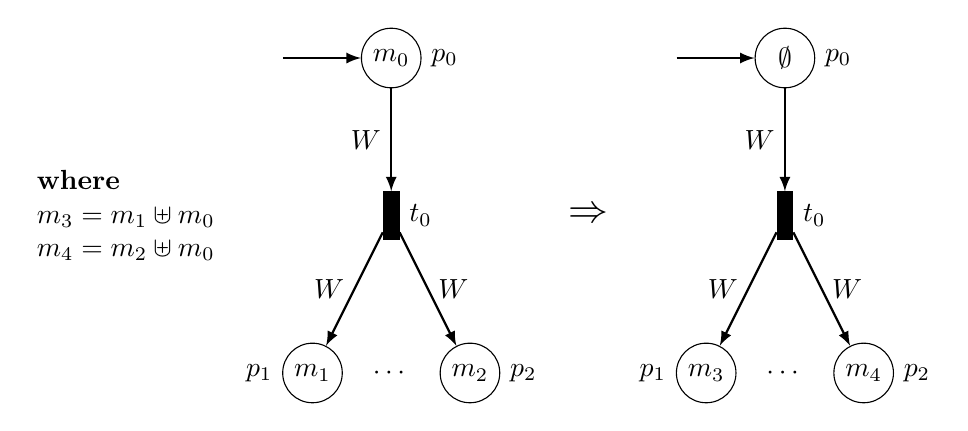
\begin{tikzpicture}
        % left side Places
        \node[place, label=right:$p_0$] (place0) at (-1,4) {$m_0$};
        \node[place, label=left:$p_1$] (place1) at (-2,0) {$m_1$};
        \node[] (empty) at (-1,0) {$\cdots$};
        \node[place, label=right:$p_2$] (place2) at (0,0) {$m_2$};

        % Left side transitions
        \node[transition,minimum height=6mm,minimum width=2mm,fill=black,label=right:$t_0$] (lTrans1) at (-1,2) {};

        % Left side invisible nodes
        \node (negIn1) at (-2.5,4) {};

        % Left side arcs between transitions and places
        \draw[-latex,thick] (place0) -- node[left] {$W$} (lTrans1);
        \draw[-latex,thick] (lTrans1) -- node [left] {$W$} (place1);
        \draw[-latex,thick] (lTrans1) -- node [right] {$W$} (place2);

        % Left side arcs to/from invisible nodes
        \draw[-latex,thick] (negIn1) -- node[above] {} (place0);

        % ================== Middle arrow ==================
        \node (arrow) at (1.5,2) {\Large$\Rightarrow$};
        \node[text width=4cm] at (-3.5,2) {\textbf{where }\\$m_3 = m_1 \uplus m_0$\\$m_4 = m_2 \uplus m_0$};
        % ==================================================

        % right side Places
        \node[place, label=right:$p_0$] (rplace0) at (4,4) {$\emptyset$};
        \node[place, label=left:$p_1$] (rplace1) at (3,0) {$m_3$};
        \node[] (empty) at (4,0) {$\cdots$};
        \node[place, label=right:$p_2$] (rplace2) at (5,0) {$m_4$};

        % right side transitions
        \node[transition,minimum height=6mm,minimum width=2mm,fill=black,label=right:$t_0$] (rTrans1) at (4,2) {};

        % right side invisible nodes
        \node (rnegIn1) at (2.5,4) {};

        % Left side arcs between transitions and places
        \draw[-latex,thick] (rplace0) -- node[left] {$W$} (rTrans1);
        \draw[-latex,thick] (rTrans1) -- node [left] {$W$} (rplace1);
        \draw[-latex,thick] (rTrans1) -- node [right] {$W$} (rplace2);

        % Left side arcs to/from invisible nodes
        \draw[-latex,thick] (rnegIn1) -- node[above] {} (rplace0);

    \end{tikzpicture}
    \vspace{5mm}

    \begin{adjustbox}{center}
        \begin{tabular}{|p{65mm}|p{60mm}|}
            \hline
            Precondition & Update \\ \hline
            Fix place $p_0$ and transition $t_0$ s.t.:
            \begin{itemize}[leftmargin=10mm]
                \item[Q1)] $p_0^\bullet = \{t_0\}$ and ${}^\bullet t_0 = \{p_0\}$
                \item[Q2)] $G(t_0) = \top$
                \item[Q3)] $(\{p_0\}\cup t^\bullet)\cap places(\varphi)=\emptyset$ and

                $(\{t_0\}\cup (t^\bullet)^\bullet)\cap transitions(\varphi)=\emptyset$

                \item[Q4)] $p_0^\circ=\emptyset$ and $(t_0^\bullet)^\circ=\emptyset$
                \item[Q5)] ${}^\circ t_0=\emptyset$
                \item[Q6)] $\exists k\in\N . k\cdot |\boxminus(p_0, t_0)| = |M_0(p_0)|$
                \item[Q7)] ${}^\bullet p_0\neq\emptyset\implies |\boxminus(p_0, t_0)|=1$
                \item[Q8)] $|\textbf{Supp}(M_0(p_0))=1|$ or\newline $\forall\vec x\in\boxminus(p_0,t_0)(\vec x)=1$
            \end{itemize}
            and for all $p\in t_0^\bullet$:
            \begin{itemize}[leftmargin=10mm]
                \item[Q8)] $\mathcal X(p) = \mathcal X(p_0) $
                \item[Q9)] $\boxminus(p_0, t_0) = \boxplus(t_0, p)$
            \end{itemize}
            &
            \begin{itemize}[leftmargin=10mm]
                \item[UQ1)] $\forall p \in t_0^\bullet . M_0'(p) \coloneqq M_0(p) \uplus M_0(p_0) $
                \item[UQ2)] $M_0'(p_0):=\emptyset$
            \end{itemize} \\ \hline
        \end{tabular}
    \end{adjustbox}
    \caption{Rule Q: Preemptive firing}
    \label{fig:rule_q_cpn}
\end{figure}

\begin{theorem}
    Rule~Q in Figure~\ref{fig:rule_q_cpn} is correct for CTL*\textbackslash X.
\end{theorem}

    \clearpage
    \section*{Rule S: Atomic free agglomeration with k-scaling (CPN)}\label{sec:rule_s_cpn}
A free agglomeration is a pre agglomeration, which does not require that the pre set of the preset of $p_0$ has a single consumer.
In turn, it is only correct for reachability with deadlocks.
The atomic free agglomeration is similar to the free agglomeration, but is able to agglomeration one consumer at a time.
See Figure~\ref{fig:rule_s_cpn} for its definition.
Rule~S also handles cases where the producer $h$ produces $k$ times more tokens than what the consumer $f_0$ consumes.
In this case, a transition $\langle h f_0^i\rangle$ is created for each $i\in [1, k]$.
Thus all relevant markings remain reachable.

\begin{theorem}
    Rule~S in Figure~\ref{fig:rule_s_cpn} is correct for reachability without deadlock.
\end{theorem}

\begin{figure}
    \centering
    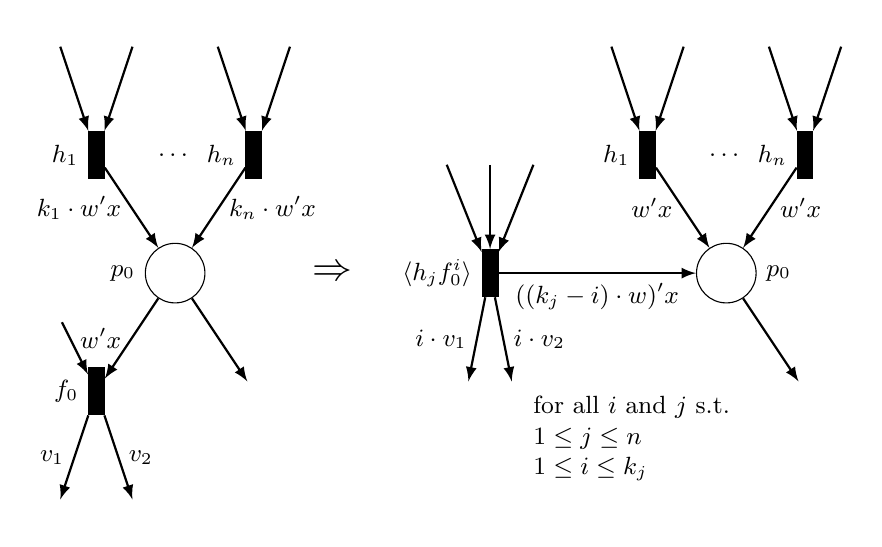
\begin{tikzpicture}
        \tikzstyle{every node}=[font=\small]
        %%% Before
        \begin{scope}[scale=0.5]
            \node[place,label=left:$p_0$] (p0) at (0,0) {};
            \node (h1pre1) at (-3,6) {};
            \node (h1pre2) at (-1,6) {};
            \node (hnpre1) at (1,6) {};
            \node (hnpre2) at (3,6) {};
            \node (f1pre) at (-3,-1) {};
            \node (f1post1) at (-3,-6) {};
            \node (f1post2) at (-1,-6) {};
            \node (fmpre) at (3,-1) {};
            \node (fmpost1) at (1,-6) {};
            \node (fmpost2) at (3,-6) {};
            \node (fm) at (2,-3) {};

            \node[transition,minimum height=6mm,minimum width=2mm,fill=black,label=left:$h_1$] (h1) at (-2,3) {};
            \node (hdots) at (0,3) {$\dots$};
            \node[transition,minimum height=6mm,minimum width=2mm,fill=black,label=left:$h_n$] (hn) at (2,3) {};
            \node[transition,minimum height=6mm,minimum width=2mm,fill=black,label=left:$f_0$] (f1) at (-2,-3) {};
            %\node (fdots) at (-2,-5) {$\dots$};
            %\node[transition,minimum height=6mm,minimum width=2mm,fill=black,label=left:$f_m$] (fm) at (2,-3) {};

            \draw[-latex,thick] (h1pre1) edge (h1);
            \draw[-latex,thick] (h1pre2) edge (h1);
            \draw[-latex,thick] (hnpre1) edge (hn);
            \draw[-latex,thick] (hnpre2) edge (hn);
            \draw[-latex,thick] (h1) edge node[left] {$k_1 \cdot w'x$} (p0);
            \draw[-latex,thick] (hn) edge node[right] {$k_n \cdot w'x$} (p0);
            \draw[-latex,thick] (p0) edge node[left] {$w'x$} (f1);
            \draw[-latex,thick] (p0) edge node[right] {} (fm);
            \draw[-latex,thick] (f1pre) edge (f1);
            \draw[-latex,thick] (f1) edge node[left] {$v_1$} (f1post1);
            \draw[-latex,thick] (f1) edge node[right] {$v_2$} (f1post2);
            %\draw[-latex,thick] (fmpre) edge (fm);
            %\draw[-latex,thick] (fm) edge (fmpost1);
            %\draw[-latex,thick] (fm) edge (fmpost2);
        \end{scope}

        \node (arrow) at (2,0) {\Large $\Rightarrow$};

        %%% After
        \begin{scope}[shift={(4,0)},scale=0.6]
        \node (p1) at (-1,2.5) {};
        \node (p2) at (0,2.5) {};
        \node (p9) at (1,2.5) {};
        \node (p3) at (1,2.5) {};
        \node (p4) at (2,2.5) {};
        \node (p10) at (3,2.5) {};
        \node (p5) at (-0.5,-2.5) {};
        \node (p6) at (0.5,-2.5) {};
        \node (p7) at (1.5,-2.5) {};
        \node (p8) at (2.5,-2.5) {};

        \node[transition,minimum height=6mm,minimum width=2mm,fill=black,label=left:$\langle h_j f_0^{i}\rangle$] (hjfi) at (0,0) {};
        \node[text width=2.5cm] (explain) at (3,-3.5) {for all $i$ and $j$ s.t. $1\leq j\leq n$\\$1 \leq i\leq k_j$};

        \draw[-latex,thick] (p1) edge (hjfi);
        \draw[-latex,thick] (p2) edge (hjfi);
        \draw[-latex,thick] (p9) edge (hjfi);
        % \draw[-latex,thick] (p3) edge (hnfm);
        % \draw[-latex,thick] (p4) edge (hnfm);
        % \draw[-latex,thick] (p10) edge (hnfm);
        \draw[-latex,thick] (hjfi) edge node[left] {$i \cdot v_1$} (p5);
        \draw[-latex,thick] (hjfi) edge node[right] {$i \cdot v_2$} (p6);
            % \draw[-latex,thick] (hnfm) edge node[left] {} (p7);
        \end{scope}
        \begin{scope}[shift={(7,0)}, scale=0.5]
        \node[place,label=right:$p_0$] (p0) at (0,0) {};
        \node (h1pre1) at (-3,6) {};
        \node (h1pre2) at (-1,6) {};
        \node (hnpre1) at (1,6) {};
        \node (hnpre2) at (3,6) {};
        %\node (f1pre) at (-3,-1) {};
        %\node (f1post1) at (-3,-6) {};
        %\node (f1post2) at (-1,-6) {};
        \node (fmpre) at (3,-1) {};
        \node (fmpost1) at (1,-6) {};
        \node (fmpost2) at (3,-6) {};
        \node (fm) at (2,-3) {};

        \node[transition,minimum height=6mm,minimum width=2mm,fill=black,label=left:$h_1$] (h1) at (-2,3) {};
        \node (hdots) at (0,3) {$\dots$};
        \node[transition,minimum height=6mm,minimum width=2mm,fill=black,label=left:$h_n$] (hn) at (2,3) {};
        %\node[transition,minimum height=6mm,minimum width=2mm,fill=black,label=left:$f_0$] (f1) at (-2,-3) {};
        %\node (fdots) at (-2,-5) {$\dots$};
        %\node[transition,minimum height=6mm,minimum width=2mm,fill=black,label=left:$f_m$] (fm) at (2,-3) {};

        \draw[-latex,thick] (h1pre1) edge (h1);
        \draw[-latex,thick] (h1pre2) edge (h1);
        \draw[-latex,thick] (hnpre1) edge (hn);
        \draw[-latex,thick] (hnpre2) edge (hn);
        \draw[-latex,thick] (h1) edge node[left] {$w'x$} (p0);
        \draw[-latex,thick] (hn) edge node[right] {$w'x$} (p0);
        %\draw[-latex,thick] (p0) edge node[left] {$W$} (f1);
        \draw[-latex,thick] (p0) edge node[right] {} (fm);
        \draw[-latex,thick] (hjfi) edge node[below] {$((k_j-i)  \cdot  w)'x$} (p0);
            %\draw[-latex,thick] (f1pre) edge (f1);
            %\draw[-latex,thick] (f1) edge node[left] {} (f1post1);
            %\draw[-latex,thick] (f1) edge node[right] {} (f1post2);
            %\draw[-latex,thick] (fmpre) edge (fm);
            %\draw[-latex,thick] (fm) edge (fmpost1);
            %\draw[-latex,thick] (fm) edge (fmpost2);
        \end{scope}
    \end{tikzpicture}
    \vspace{5mm}
    \begin{adjustbox}{center}
        \begin{tabular}{|p{70mm}|p{70mm}|} \hline
        Precondition & Update \\ \hline
        Fix place $p_0$ and transition $f_0$ s.t.:
        \begin{itemize}[leftmargin=10mm]
            \item[S1)] $(\{p_0\} \cap places(\varphi) = \emptyset$
            \item[S2)] $({}^\bullet p_0 \cup p_0^\bullet \cup ({}^\bullet {}^\bullet p_0)^\bullet) \cap transitions(\varphi) = \emptyset$
            \item[S3)] $M_0(p_0)=\emptyset$
            \item[S4)] $^\bullet p_0 \cap p_0^\bullet = \emptyset$
            \item[S5)] $f_0 \in p_0^\bullet$
            \item[S6)] $|\textbf{Supp}(\boxminus(p_0, f_0))| = 1$
        \end{itemize}
        \hspace{2mm}
        and for all $h\in{}^\bullet p$:
        \begin{itemize}[leftmargin=10mm]
            \item[S7)] $h^\bullet=\{p_0\}$
            \item[S8)] ${}^\bullet h \cap places(\varphi) = \emptyset$
            \item[S9)] $p_0^\circ = {}^\circ h = ({}^\bullet h)^\circ = \emptyset$
            %\item[S10)] $|\boxplus(h, p_0)| = |\boxminus(p_0, f_0)|$
            \item[S10)] $|\boxplus(h, p_0)| = k * |\boxminus(p_0, f_0)|$
            \item[S11)] $k > 1 \implies{}^\bullet f_0 = \{p_0\}$
            \item[S12)] $k > 1 \implies (f_0^\bullet)^\circ = \emptyset$
        \end{itemize}
        And for each variable $v \in ((\boxplus(h, p_0) \cup \boxminus(p_0, f_0)) \cap (\textbf{Vars}(G(h)) \cup \textbf{Vars}(G(f_0)))$\newline
        there exists a $p$ \in P\backslash $\{p_0\}$ such that:
        \begin{itemize}[leftmargin=13mm]
            \item[S13)] $v \in (\textbf{Vars}(\boxplus(h, p)) \cup \textbf{Vars}(\boxminus(p, f_0)))$
        \end{itemize}

        &
        For all $h\in{}^\bullet p_0$, create a transition $\langle hf\rangle$ s.t. for all $p\in P\setminus\{p_0\}$, for all $i \in [1,k]$ for the $k$ such that $|\boxplus(h, p_0)| = k*|\boxminus(p_0, f_0)|$:
        \begin{itemize}[leftmargin=10mm]
            \item[US1)] For all $v \in \textbf{Vars}(f_0)$, $rename(f_0,v,v')$ with some $v' \in \textbf{Var}_{\mathcal{X}(p)}\backslash\textbf{Vars}(h)$
            \item[US2)] $\boxminus(p,\langle hf_0^i\rangle):=\boxminus(p,h)\uplus \boxminus(p,f_0)$
            \item[US3)] $\boxplus(\langle hf_0^i\rangle,p):= i * \boxplus(f_0,p)$

                $\boxplus(\langle hf_0^i\rangle,p_0):= (k-i) * \boxminus(p_0,f_0)$

            \item[US4)] $G(\langle hf_0^i\rangle):= G(h) \land G(f_0)$
            \item[US5)] $I(\langle hf_0^i\rangle):= I(f_0)$
            %\item[US6)] Given that $\boxplus(h,p_0) = \{\langle x_1, x_2, \dots, x_n \rangle\}$ and $\boxminus(p_0, f_0) = \{\langle y_1, y_2, \dots, y_n \rangle\}$, $G(\langle hf \rangle) \land \bigwedge_{i\in[1,n]} (x_i = y_i)$
            \item[US6)] Given that $\boxplus(h,p_0) = \{\langle x_1, x_2, \dots, x_n \rangle\}$ and $\boxminus(p_0, f_0) = \{\langle y_1, y_2, \dots, y_n \rangle\}$\newline
            For $j\in[1,n]$\newline
            Let $l$ be the smallest number s.t.\ $x_l = x_i$ holds:\newline
            $rename(\langle hf_0^i \rangle, x_j, y_l), rename(\langle hf_0^i \rangle, y_j, y_l)$
            %\item[US-optional)] For every expression of the form $x = y$ in $G(\langle hf \rangle)$, replace all instances of variable $x$ in the arcs and guards of $\langle hf \rangle$ with variable $y$
        \end{itemize}
        and
        \begin{itemize}[leftmargin=10mm]
            \item[US7)] Remove $f_0$
            \item[US8)] If $p_0^\bullet = \emptyset$, remove $p_0$ and all transitions in ${}^\bullet p_0\setminus transitions(\varphi)$
        \end{itemize} \\ \hline
        \end{tabular}
    \end{adjustbox}
    \caption{Rule S: Atomic free agglomeration with k-scaled}
    \label{fig:rule_s_cpn}
\end{figure}

    \clearpage
    \section*{Rule T: Pre agglomeration (CPN)}\label{sec:rule_t_cpn}
Rule~T in Figure~\ref{fig:rule_t_cpn} is a pre agglomeration.
In a pre agglomeration $h\in{}^\bullet p_0$ is invisible to the query and once enabled, it stays enabled.
Hence, it can be delayed until an $f\in p_0^\bullet$ needs it.
Thus Rule~T creates a transition $\langle h f\rangle$ for every pair $h\in{}^\bullet p_0$ and $f\in p_0^\bullet$.

\begin{theorem}
    Rule~T described in Figure~\ref{fig:rule_t_cpn} is correct for LTL\textbackslash X.
\end{theorem}

\begin{figure}[h!]
    \centering
    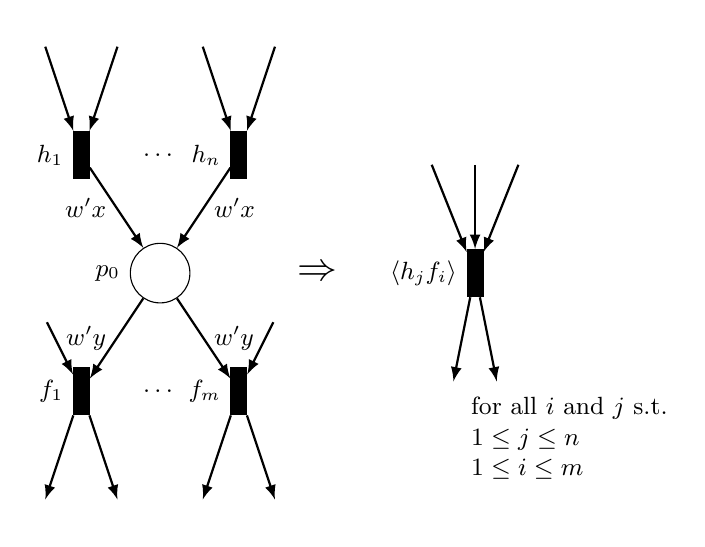
\begin{tikzpicture}
        \tikzstyle{every node}=[font=\small]
        %%% Before
        \begin{scope}[scale=0.5]
            \node[place,label=left:$p_0$] (p0) at (0,0) {};
            \node (h1pre1) at (-3,6) {};
            \node (h1pre2) at (-1,6) {};
            \node (hnpre1) at (1,6) {};
            \node (hnpre2) at (3,6) {};
            \node (f1pre) at (-3,-1) {};
            \node (f1post1) at (-3,-6) {};
            \node (f1post2) at (-1,-6) {};
            \node (fmpre) at (3,-1) {};
            \node (fmpost1) at (1,-6) {};
            \node (fmpost2) at (3,-6) {};
            \node (fm) at (2,-3) {};

            \node[transition,minimum height=6mm,minimum width=2mm,fill=black,label=left:$h_1$] (h1) at (-2,3) {};
            \node (hdots) at (0,3) {$\dots$};
            \node (fdots) at (0,-3) {$\dots$};
            \node[transition,minimum height=6mm,minimum width=2mm,fill=black,label=left:$h_n$] (hn) at (2,3) {};
            \node[transition,minimum height=6mm,minimum width=2mm,fill=black,label=left:$f_1$] (f1) at (-2,-3) {};
            \node[transition,minimum height=6mm,minimum width=2mm,fill=black,label=left:$f_m$] (fm) at (2,-3) {};
            %\node (fdots) at (-2,-5) {$\dots$};
            %\node[transition,minimum height=6mm,minimum width=2mm,fill=black,label=left:$f_m$] (fm) at (2,-3) {};

            \draw[-latex,thick] (h1pre1) edge (h1);
            \draw[-latex,thick] (h1pre2) edge (h1);
            \draw[-latex,thick] (hnpre1) edge (hn);
            \draw[-latex,thick] (hnpre2) edge (hn);
            \draw[-latex,thick] (h1) edge node[left] {$w{}'x$} (p0);
            \draw[-latex,thick] (hn) edge node[right] {$w{}'x$} (p0);
            \draw[-latex,thick] (p0) edge node[left] {$w{}'y$} (f1);
            \draw[-latex,thick] (p0) edge node[right] {$w{}'y$} (fm);
            \draw[-latex,thick] (f1pre) edge (f1);
            \draw[-latex,thick] (f1) edge(f1post1);
            \draw[-latex,thick] (f1) edge (f1post2);
            \draw[-latex,thick] (fmpre) edge (fm);
            \draw[-latex,thick] (fm) edge (fmpost1);
            \draw[-latex,thick] (fm) edge (fmpost2);
        \end{scope}

        \node (arrow) at (2,0) {\Large $\Rightarrow$};

        %%% After
        \begin{scope}[shift={(4,0)},scale=0.6]
        \node (p1) at (-1,2.5) {};
        \node (p2) at (0,2.5) {};
        \node (p9) at (1,2.5) {};
%            \node (p3) at (1,2.5) {};
%            \node (p4) at (2,2.5) {};
%            \node (p10) at (3,2.5) {};
        \node (p5) at (-0.5,-2.5) {};
        \node (p6) at (0.5,-2.5) {};
%            \node (p7) at (1.5,-2.5) {};
%            \node (p8) at (2.5,-2.5) {};

        \node[transition,minimum height=6mm,minimum width=2mm,fill=black,label=left:$\langle h_j f_i \rangle$] (hjfi) at (0,0) {};
        \node[text width=2.5cm] (explain) at (2,-3.5) {for all $i$ and $j$ s.t. $1\leq j\leq n$\\$1 \leq i\leq m$};

        \draw[-latex,thick] (p1) edge (hjfi);
        \draw[-latex,thick] (p2) edge (hjfi);
        \draw[-latex,thick] (p9) edge (hjfi);
        % \draw[-latex,thick] (p3) edge (hnfm);
        % \draw[-latex,thick] (p4) edge (hnfm);
        % \draw[-latex,thick] (p10) edge (hnfm);
        \draw[-latex,thick] (hjfi) edge (p5);
        \draw[-latex,thick] (hjfi) edge (p6);
            % \draw[-latex,thick] (hnfm) edge node[left] {} (p7);
        \end{scope}
%        \begin{scope}[shift={(7,0)}, scale=0.5]
%%            \node[place,label=right:$p_0$] (p0) at (0,0) {};
%%            \node (h1pre1) at (-3,6) {};
%%            \node (h1pre2) at (-1,6) {};
%%            \node (hnpre1) at (1,6) {};
%%            \node (hnpre2) at (3,6) {};
%%            %\node (f1pre) at (-3,-1) {};
%%            %\node (f1post1) at (-3,-6) {};
%%            %\node (f1post2) at (-1,-6) {};
%%            \node (fmpre) at (3,-1) {};
%%            \node (fmpost1) at (1,-6) {};
%%            \node (fmpost2) at (3,-6) {};
%%            \node (fm) at (2,-3) {};
%
%%            \node[transition,minimum height=6mm,minimum width=2mm,fill=black,label=left:$h_1$] (h1) at (-2,3) {};
%%            \node (hdots) at (0,3) {$\dots$};
%%            \node[transition,minimum height=6mm,minimum width=2mm,fill=black,label=left:$h_n$] (hn) at (2,3) {};
%            %\node[transition,minimum height=6mm,minimum width=2mm,fill=black,label=left:$f_0$] (f1) at (-2,-3) {};
%            %\node (fdots) at (-2,-5) {$\dots$};
%            %\node[transition,minimum height=6mm,minimum width=2mm,fill=black,label=left:$f_m$] (fm) at (2,-3) {};
%
%            \draw[-latex,thick] (h1pre1) edge (h1);
%            \draw[-latex,thick] (h1pre2) edge (h1);
%            \draw[-latex,thick] (hnpre1) edge (hn);
%            \draw[-latex,thick] (hnpre2) edge (hn);
%            \draw[-latex,thick] (h1) edge node[left] {$w'x$} (p0);
%            \draw[-latex,thick] (hn) edge node[right] {$w'x$} (p0);
%            %\draw[-latex,thick] (p0) edge node[left] {$W$} (f1);
%            \draw[-latex,thick] (p0) edge node[right] {} (fm);
%            \draw[-latex,thick] (hjfi) edge node[below] {$((k_j-i)  \cdot  w)'x$} (p0);
%            %\draw[-latex,thick] (f1pre) edge (f1);
%            %\draw[-latex,thick] (f1) edge node[left] {} (f1post1);
%            %\draw[-latex,thick] (f1) edge node[right] {} (f1post2);
%            %\draw[-latex,thick] (fmpre) edge (fm);
%            %\draw[-latex,thick] (fm) edge (fmpost1);
%            %\draw[-latex,thick] (fm) edge (fmpost2);
%        \end{scope}
    \end{tikzpicture}
    \vspace{5mm}
    \begin{adjustbox}{center}
        \begin{tabular}{|p{70mm}|p{70mm}|} \hline
        Precondition & Update \\ \hline
        Fix place $p_0$ s.t.:
        \begin{itemize}[leftmargin=9mm]
            \item[T1)] $(\{p_0\} \cap places(\varphi) = \emptyset$
            \item[T2)] $(p_0^\bullet \cup {}^\bullet p_0) \cap transitions(\varphi) = \emptyset$
            \item[T3)] $M_0(p_0)=\emptyset$
            \item[T4)] $^\bullet p_0 \cap p_0^\bullet = \emptyset$

        \end{itemize}
        \hspace{2mm}
        and for all $h\in{}^\bullet p_0$:
        \begin{itemize}[leftmargin=9mm]
            \item[T5)] $(^\bullet h)^\bullet = \{h\}$
            \item[T6)] $h^\bullet=\{p_0\}$
            \item[T7)] ${}^\bullet h \cap places(\varphi) = \emptyset$
            \item[T8)] $p_0^\circ = {}^\circ h = ({}^\bullet h)^\circ = \emptyset$
        \end{itemize}
        \hspace{2mm}
        and for all $f\in p_0^\bullet$
        \begin{itemize}[leftmargin=11mm]
            \item[T9)] $|\textbf{Supp}(\boxplus(h, p_0))| = |\textbf{Supp}(\boxminus(p_0, f))| = 1$
            \item[T10)] $|\boxplus(h, p_0)| = |\boxminus(p_0,f)|$
        \end{itemize}
        &
        For all $h\in{}^\bullet p$, for all $f\in p^\bullet$, create a transition $\langle hf\rangle$ s.t.\ for all $p\in P\setminus\{p_0\}$:
        \begin{itemize}[leftmargin=10mm]
            \item[UT1)] For all $v \in\textbf{Vars}(f)$, $rename(f,v,v')$ with some $v' \in\textbf{Vars}_{\mathcal{X}(p)}\backslash\textbf{Vars}(h)$
            \item[UT2)] $\boxminus(p,\langle hf\rangle) := \boxminus(p,h)\uplus\boxminus(p,f)$
            \item[UT3)] $\boxplus(\langle hf\rangle,p) := \boxplus(f,p)$
            \item[UT4)] $G(\langle hf\rangle) := G(h) \land G(f)$
            \item[UT5)] $I(\langle hf\rangle) := I(f)$
            %\item[UT6)] Given that $\boxplus(h,p_0) = \{\langle x_1, x_2, \dots, x_n \rangle\}$ and $\boxminus(p_0, f) = \{\langle y_1, y_2, \dots, y_n \rangle\}$, $G(\langle hf \rangle) \land \bigwedge_{i\in[1,n]} (x_i = y_i)$
            \item[UT6)] Given that $\boxplus(h,p_0) = w{}'\langle x_1, x_2, \dots, x_n \rangle$ and $\boxminus(p_0, f_0) = w{}'\langle y_1, y_2, \dots, y_n \rangle$\newline
            For $i\in[1,n]$\newline
            Let $a$ be the smallest index s.t.\ $x_a = x_i$ holds:\newline
            $rename(\langle hf \rangle, x_i, y_a)$\newline
            $rename(\langle hf \rangle, y_i, y_a)$
        \end{itemize}
        and after all such transitions are made:
        \begin{itemize}[leftmargin=10mm]
            \item[UT7)] Remove $p^\bullet$, ${}^\bullet p_0$, and $p_0$
        \end{itemize} \\ \hline
        \end{tabular}
    \end{adjustbox}
    \caption{Rule T: Pre agglomeration}
    \label{fig:rule_t_cpn}
\end{figure}

    \clearpage
    \section*{Rule U: Atomic free agglomeration (CPN)}\label{sec:rule_u_cpn}
Rule~U is a atomic free agglomeration similar to Rule~S.
However, it restricts $k=1$.
See Figure~\ref{fig:rule_u_cpn} for the definition of Rule~U.

\begin{theorem}
    Rule~U in Figure~\ref{fig:rule_u_cpn} is correct for reachability without deadlock.
\end{theorem}

\begin{figure}
    \centering
    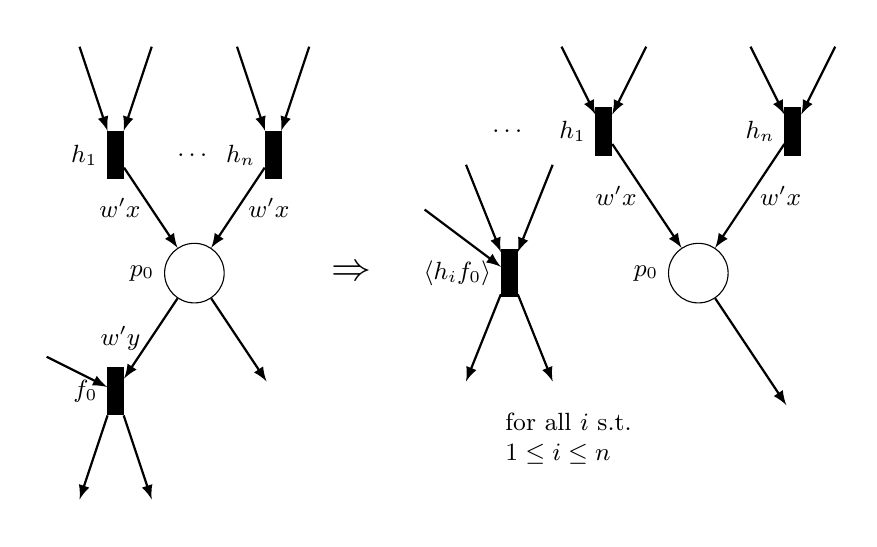
\begin{tikzpicture}
        \tikzstyle{every node}=[font=\small]
        %%% Before
        \begin{scope}[scale=0.5]
            \node[place,label=left:$p_0$] (p0) at (0,0) {};
            \node (h1pre1) at (-3,6) {};
            \node (h1pre2) at (-1,6) {};
            \node (hnpre1) at (1,6) {};
            \node (hnpre2) at (3,6) {};
            \node (f1pre) at (-4,-2) {};
            \node (f1post1) at (-3,-6) {};
            \node (f1post2) at (-1,-6) {};
            \node (fmpre) at (3,-1) {};
            \node (fmpost1) at (1,-6) {};
            \node (fmpost2) at (3,-6) {};
            \node (fm) at (2,-3) {};

            \node[transition,minimum height=6mm,minimum width=2mm,fill=black,label=left:$h_1$] (h1) at (-2,3) {};
            \node (hdots) at (0,3) {$\dots$};
            \node[transition,minimum height=6mm,minimum width=2mm,fill=black,label=left:$h_n$] (hn) at (2,3) {};
            \node[transition,minimum height=6mm,minimum width=2mm,fill=black,label=left:$f_0$] (f1) at (-2,-3) {};
            %\node (fdots) at (-2,-5) {$\dots$};
            %\node[transition,minimum height=6mm,minimum width=2mm,fill=black,label=left:$f_m$] (fm) at (2,-3) {};

            \draw[-latex,thick] (h1pre1) edge (h1);
            \draw[-latex,thick] (h1pre2) edge (h1);
            \draw[-latex,thick] (hnpre1) edge (hn);
            \draw[-latex,thick] (hnpre2) edge (hn);
            \draw[-latex,thick] (h1) edge node[left] {$w'x$} (p0);
            \draw[-latex,thick] (hn) edge node[right] {$w'x$} (p0);
            \draw[-latex,thick] (p0) edge node[left] {$w'y$} (f1);
            \draw[-latex,thick] (p0) edge node[right] {} (fm);
            \draw[-latex,thick] (f1pre) edge (f1);
            \draw[-latex,thick] (f1) edge (f1post1);
            \draw[-latex,thick] (f1) edge (f1post2);
            %\draw[-latex,thick] (fmpre) edge (fm);
            %\draw[-latex,thick] (fm) edge (fmpost1);
            %\draw[-latex,thick] (fm) edge (fmpost2);
        \end{scope}


        \node (arrow) at (2,0) {\Large $\Rightarrow$};

        %%% After
        \begin{scope}[shift={(4,0)},scale=0.6]

        \node[place,label=left:$p_0$] (p0) at (4,0) {};
        \node (h1pre1) at (1,5) {};
        \node (h1pre2) at (3,5) {};
        \node (hnpre1) at (5,5) {};
        \node (hnpre2) at (7,5) {};


        \node (p1) at (-1,2.5) {};
        \node (p2) at (-2,1.5) {};
        \node (p9) at (1,2.5) {};
        \node (p5) at (-1,-2.5) {};
        \node (p6) at (1,-2.5) {};

        \node[transition,minimum height=6mm,minimum width=2mm,fill=black,label=left:$h_1$] (h1) at (2,3) {};
        \node (hdots) at (0,3) {$\dots$};
        \node (falt) at (6,-3) {};
        \node[transition,minimum height=6mm,minimum width=2mm,fill=black,label=left:$h_n$] (hn) at (6,3) {};
        \node[transition,minimum height=6mm,minimum width=2mm,fill=black,label=left:$\langle h_i f_0 \rangle$] (hjfi) at (0,0) {};
        \node[text width=2.5cm] (explain) at (2,-3.5) {for all $i$ s.t.\\ $1\leq i\leq n$};

        \draw[-latex,thick] (h1pre1) edge (h1);
        \draw[-latex,thick] (h1pre2) edge (h1);
        \draw[-latex,thick] (hnpre1) edge (hn);
        \draw[-latex,thick] (hnpre2) edge (hn);
        \draw[-latex,thick] (h1) edge node[left] {$w'x$} (p0);
        \draw[-latex,thick] (hn) edge node[right] {$w'x$} (p0);

        \draw[-latex,thick] (p1) edge (hjfi);
        \draw[-latex,thick] (p2) edge (hjfi);
        \draw[-latex,thick] (p9) edge (hjfi);
        % \draw[-latex,thick] (p3) edge (hnfm);
        % \draw[-latex,thick] (p4) edge (hnfm);
        % \draw[-latex,thick] (p10) edge (hnfm);
        \draw[-latex,thick] (hjfi) edge (p5);
        \draw[-latex,thick] (hjfi) edge (p6);
        \draw[-latex,thick] (p0) edge (falt);
            % \draw[-latex,thick] (hnfm) edge node[left] {} (p7);
        \end{scope}
    \end{tikzpicture}
    \vspace{5mm}
    \begin{adjustbox}{center}
        \begin{tabular}{|p{70mm}|p{70mm}|} \hline
        Precondition & Update \\ \hline
        Fix place $p_0$ and transition $f_0$ s.t.:
        \begin{itemize}[leftmargin=10mm]
            \item[U1)] $(\{p_0\} \cap places(\varphi) = \emptyset$
            \item[U2)] $({}^\bullet p_0 \cup p_0^\bullet \cup ({}^\bullet {}^\bullet p_0)^\bullet) \cap transitions(\varphi) = \emptyset$
            \item[U3)] $M_0(p_0)=\emptyset$
            \item[U4)] $^\bullet p_0 \cap p_0^\bullet = \emptyset$
            \item[U5)] $f_0 \in p_0^\bullet$
        \end{itemize}
        \hspace{2mm}
        and for all $h\in{}^\bullet p$:
        \begin{itemize}[leftmargin=10mm]
            \item[U6)] $|\textbf{Supp}(\boxplus(h, p_0))| = |\textbf{Supp}(\boxminus(p_0, f_0))| = 1$
            \item[U7)] $h^\bullet=\{p_0\}$
            \item[U8)] ${}^\bullet h \cap places(\varphi) = \emptyset$
            \item[U9)] $p_0^\circ = {}^\circ h = ({}^\bullet h)^\circ = \emptyset$
            \item[U10)] $|\boxplus(h, p_0)| = |\boxminus(p_0, f_0)|$
            %\item[U10)] $|\boxplus(h, p_0)| = k * |\boxminus(p_0, f_0)|$
            %\item[U11)] $k > 1 \implies{}^\bullet f_0 = \{p_0\}$
            %\item[U12)] $k > 1 \implies (f_0^\bullet)^\circ = \emptyset$
        \end{itemize}
%    And for each variable $v \in ((\boxplus(h, p_0) \cup \boxminus(p_0, f_0)) \cap (\textbf{Vars}(G(h)) \cup \textbf{Vars}(G(f_0)))$\newline
%    there exists a $p$ \in P\backslash $\{p_0\}$ such that:
%    \begin{itemize}[leftmargin=13mm]
%        \item[U11)] $v \in (\textbf{Vars}(\boxplus(h, p)) \cup \textbf{Vars}(\boxminus(p, f_0)))$
%    \end{itemize}

        &
        For all $h\in{}^\bullet p_0$, create a transition $\langle hf\rangle$ s.t. for all $p\in P\setminus\{p_0\}$:
        \begin{itemize}[leftmargin=10mm]
            \item[UU1)] For all $v \in Vars(f_0)$, $rename(f_0,v,v')$ with some $v' \in Var_{\mathcal{X}(p)}\backslash Vars(h)$
            \item[UU2)] $\boxminus(p,\langle hf\rangle)=\boxminus(p,h)\uplus \boxminus(p,f_0)$
            \item[UU3)] $\boxplus(\langle hf\rangle,p)=\boxplus(f_0,p)$
            \item[UU4)] $G(\langle hf\rangle) = G(h) \land G(f_0)$
            \item[UU5)] $I(\langle hf\rangle) = I(f_0)$
            %\item[UU6)] Given that $\boxplus(h,p_0) = \{\langle x_1, x_2, \dots, x_n \rangle\}$ and $\boxminus(p_0, f_0) = \{\langle y_1, y_2, \dots, y_n \rangle\}$, $G(\langle hf \rangle) \land \bigwedge_{i\in[1,n]} (x_i = y_i)$
            \item[UU6)] Given that $\boxplus(h,p_0) = w{}'\langle x_1, x_2, \dots, x_n \rangle$ and $\boxminus(p_0, f_0) = w{}'\langle y_1, y_2, \dots, y_n \rangle$\newline
            For $i\in[1,n]$\newline
            Let $a$ be the minimum value for which $x_a = x_i$ holds:\newline
            $rename(\langle hf \rangle, x_i, y_a), rename(\langle hf \rangle, y_i, y_a)$
            %\item[UU-optional)] For every expression of the form $x = y$ in $G(\langle hf \rangle)$, replace all instances of variable $x$ in the arcs and guards of $\langle hf \rangle$ with variable $y$
        \end{itemize}
        and
        \begin{itemize}[leftmargin=10mm]
            \item[UU7)] Remove $f_0$
            \item[UU8)] If $p_0^\bullet = \emptyset$, remove $p_0$ and all transitions in ${}^\bullet p_0\setminus transitions(\varphi)$
        \end{itemize} \\ \hline
        \end{tabular}
    \end{adjustbox}
    \caption{Rule U: Atomic free agglomeration}
    \label{fig:rule_u_cpn}
\end{figure}

\end{document}
